% !TeX spellcheck = hu_HU
% !TeX encoding = UTF-8
% !TeX program = xelatex
% TODO Change language to en_GB (recommended) or en_US for English documents
\documentclass[11pt,a4paper,oneside]{report}             % Single-side
%\documentclass[11pt,a4paper,twoside,openright]{report}  % Duplex

% thanks to http://tex.stackexchange.com/a/47579/71109
\usepackage{ifxetex}
\usepackage{ifluatex}
\newif\ifxetexorluatex % a new conditional starts as false
\ifnum 0\ifxetex 1\fi\ifluatex 1\fi>0
   \xetexorluatextrue
\fi

\ifxetexorluatex
  \usepackage{fontspec}
\else
  \usepackage[T1]{fontenc}
  \usepackage[utf8]{inputenc}
  \usepackage[lighttt]{lmodern}
\fi

\usepackage[magyar]{babel} % Alapértelmezés szerint utoljára definiált nyelv lesz aktív, de később külön beállítjuk az aktív nyelvet.

%\usepackage{cmap}
\usepackage{amsfonts,amsmath,amssymb} % Mathematical symbols.
%\usepackage[ruled,boxed,resetcount,linesnumbered]{algorithm2e} % For pseudocodes. % beware: this is not compatible with LuaLaTeX, see http://tex.stackexchange.com/questions/34814/lualatex-and-algorithm2e
\usepackage{booktabs} % For publication quality tables for LaTeX
\usepackage{graphicx}

%\usepackage{fancyhdr}
%\usepackage{lastpage}

\usepackage{anysize}
%\usepackage{sectsty}
\usepackage{setspace} % For setting line spacing

\usepackage[unicode]{hyperref} % For hyperlinks in the generated document.
\usepackage{xcolor}
\usepackage{listings} % For source code snippets.

\usepackage[amsmath,thmmarks]{ntheorem} % Theorem-like environments.

\usepackage[hang]{caption}

\singlespacing

\newcommand{\selecthungarian}{
	\selectlanguage{magyar}
	\setlength{\parindent}{2em}
	\setlength{\parskip}{0em}
	\frenchspacing
}

\newcommand{\selectenglish}{
	\selectlanguage{english}
	\setlength{\parindent}{0em}
	\setlength{\parskip}{0.5em}
	\nonfrenchspacing
	\renewcommand{\figureautorefname}{Figure}
	\renewcommand{\tableautorefname}{Table}
	\renewcommand{\partautorefname}{Part}
	\renewcommand{\chapterautorefname}{Chapter}
	\renewcommand{\sectionautorefname}{Section}
	\renewcommand{\subsectionautorefname}{Section}
	\renewcommand{\subsubsectionautorefname}{Section}
}

\usepackage[numbers]{natbib}
\usepackage{xspace}


%TODO Set the main variables
\newcommand{\vikszerzoVezeteknev}{Fehér}
\newcommand{\vikszerzoKeresztnev}{János}

\newcommand{\vikkonzulensAMegszolitas}{dr.~}
\newcommand{\vikkonzulensAVezeteknev}{Ekler}
\newcommand{\vikkonzulensAKeresztnev}{Péter}

\newcommand{\vikcim}{Online könyvkölcsönző alkalmazás készítése a Simonyi Károly Szakkollégium számára} % Cím
\newcommand{\viktanszek}{\bmeaut} % Tanszék
\newcommand{\vikdoktipus}{\bsc} % Dokumentum típusa (\bsc vagy \msc)
\newcommand{\vikmunkatipusat}{szakdolgozatot} % a "hallgató nyilatkozat" részhez: szakdolgozatot vagy diplomatervet

%--------------------------------------------------------------------------------------
% TDK-specifikus változók
%--------------------------------------------------------------------------------------
\newcommand{\tdkszerzoB}{Második Szerző} % Második szerző neve; hagyd üresen, ha egyedül írtad a TDK-t.
\newcommand{\tdkev}{2014} % A dolgozat írásának éve (pl. "2014") (Ez OTDK-nál eltérhet az aktuális évtől.)

% További adatok az OTDK címlaphoz (BME-s TDK-hoz nem kell kitölteni)
\newcommand{\tdkevfolyamA}{IV} % Első szerző évfolyama, római számmal (pl. IV).
\newcommand{\tdkevfolyamB}{III} % Második szerző évfolyama, római számmal (pl. III).
\newcommand{\tdkkonzulensbeosztasA}{egyetemi tanár} % Első konzulens beosztása (pl. egyetemi docens)
\newcommand{\tdkkonzulensbeosztasB}{doktorandusz} % Második konzulens beosztása (pl. egyetemi docens)

\newcommand{\szerzoMeta}{\vikszerzoVezeteknev{} \vikszerzoKeresztnev} % egy szerző esetén
%\newcommand{\szerzoMeta}{\vikszerzoVezeteknev{} \vikszerzoKeresztnev, \tdkszerzoB} % két szerző esetén

%TODO Language configuration -- choose one
% Beállítások magyar nyelvű dolgozathoz
%--------------------------------------------------------------------------------------
% Elnevezések
%--------------------------------------------------------------------------------------
\newcommand{\bme}{Budapesti Műszaki és Gazdaságtudományi Egyetem}
\newcommand{\vik}{Villamosmérnöki és Informatikai Kar}

\newcommand{\bmemit}{Méréstechnika és Információs Rendszerek Tanszék}

\newcommand{\keszitette}{Készítette}
\newcommand{\konzulens}{Konzulens}

\newcommand{\bsc}{Szakdolgozat}
\newcommand{\msc}{Diplomaterv}
\newcommand{\tdk}{TDK dolgozat}
\newcommand{\bsconlab}{BSc Önálló laboratórium}
\newcommand{\msconlabi}{MSc Önálló laboratórium 1.}
\newcommand{\msconlabii}{MSc Önálló laboratórium 2.}

\newcommand{\pelda}{Példa}
\newcommand{\definicio}{Definíció}
\newcommand{\tetel}{Tétel}

\newcommand{\bevezetes}{Bevezetés}
\newcommand{\koszonetnyilvanitas}{Köszönetnyilvánítás}
\newcommand{\fuggelek}{Függelék}

% Opcionálisan átnevezhető címek
%\addto\captionsmagyar{%
%\renewcommand{\listfigurename}{Saját ábrajegyzék cím}
%\renewcommand{\listtablename}{Saját táblázatjegyzék cím}
%\renewcommand{\bibname}{Saját irodalomjegyzék név}
%}

\newcommand{\szerzo}{\vikszerzoVezeteknev{} \vikszerzoKeresztnev}
\newcommand{\vikkonzulensA}{\vikkonzulensAMegszolitas\vikkonzulensAVezeteknev{} \vikkonzulensAKeresztnev}
\newcommand{\vikkonzulensB}{\vikkonzulensBMegszolitas\vikkonzulensBVezeteknev{} \vikkonzulensBKeresztnev}
\newcommand{\vikkonzulensC}{\vikkonzulensCMegszolitas\vikkonzulensCVezeteknev{} \vikkonzulensCKeresztnev}

\newcommand{\selectthesislanguage}{\selecthungarian}

\bibliographystyle{huplain}

\def\lstlistingname{lista}

\newcommand{\appendixnumber}{6}  % a fofejezet-szamlalo az angol ABC 6. betuje (F) lesz

% Settings for English documents
% %--------------------------------------------------------------------------------------
% Elnevezések
%--------------------------------------------------------------------------------------
\newcommand{\bme}{Budapest University of Technology and Economics}
\newcommand{\vik}{Faculty of Electrical Engineering and Informatics}

\newcommand{\bmeaut}{Department of Automation and Applied Informatics}

\newcommand{\keszitette}{Author}
\newcommand{\konzulens}{Advisor}

\newcommand{\bsc}{Bachelor's Thesis}
\newcommand{\msc}{Master's Thesis}
\newcommand{\tdk}{Scientific Students' Association Report}
\newcommand{\bsconlab}{BSc Project Laboratory}
\newcommand{\msconlabi}{MSc Project Laboratory 1}
\newcommand{\msconlabii}{MSc Project Laboratory 2}

\newcommand{\pelda}{Example}
\newcommand{\definicio}{Definition}
\newcommand{\tetel}{Theorem}

\newcommand{\bevezetes}{Introduction}
\newcommand{\koszonetnyilvanitas}{Acknowledgements}
\newcommand{\fuggelek}{Appendix}

% Optional custom titles
%\addto\captionsenglish{%
%\renewcommand*{\listfigurename}{Your list of figures title}
%\renewcommand*{\listtablename}{Your list of tables title}
%\renewcommand*{\bibname}{Your bibliography title}
%}

\newcommand{\szerzo}{\vikszerzoKeresztnev{} \vikszerzoVezeteknev}
\newcommand{\vikkonzulensA}{\vikkonzulensAMegszolitas\vikkonzulensAKeresztnev{} \vikkonzulensAVezeteknev}

\newcommand{\selectthesislanguage}{\selectenglish}

\bibliographystyle{plainnat}

\newcommand{\ie}{i.e.\@\xspace}
\newcommand{\Ie}{I.e.\@\xspace}
\newcommand{\eg}{e.g.\@\xspace}
\newcommand{\Eg}{E.g.\@\xspace}
\newcommand{\etal}{et al.\@\xspace}
\newcommand{\etc}{etc.\@\xspace}
\newcommand{\vs}{vs.\@\xspace}
\newcommand{\viz}{viz.\@\xspace} % videlicet
\newcommand{\cf}{cf.\@\xspace} % confer
\newcommand{\Cf}{Cf.\@\xspace}
\newcommand{\wrt}{w.r.t.\@\xspace} % with respect to
\newcommand{\approximately}{approx.\@\xspace}

\newcommand{\appendixnumber}{1}  % a fofejezet-szamlalo az angol ABC 1. betuje (A) lesz


%--------------------------------------------------------------------------------------
% Page layout setup
%--------------------------------------------------------------------------------------
% we need to redefine the pagestyle plain
% another possibility is to use the body of this command without \fancypagestyle
% and use \pagestyle{fancy} but in that case the special pages
% (like the ToC, the References, and the Chapter pages)remain in plane style

\pagestyle{plain}
\marginsize{35mm}{25mm}{15mm}{15mm}

\setcounter{tocdepth}{3}
%\sectionfont{\large\upshape\bfseries}
\setcounter{secnumdepth}{3}

\sloppy % Margón túllógó sorok tiltása.
\widowpenalty=10000 \clubpenalty=10000 %A fattyú- és árvasorok elkerülése
\def\hyph{-\penalty0\hskip0pt\relax} % Kötőjeles szavak elválasztásának engedélyezése


%--------------------------------------------------------------------------------------
% Setup hyperref package
%--------------------------------------------------------------------------------------
\hypersetup{
    % bookmarks=true,            % show bookmarks bar?
    unicode=true,              % non-Latin characters in Acrobat's bookmarks
    pdftitle={\vikcim},        % title
    pdfauthor={\szerzoMeta},    % author
    pdfsubject={\vikdoktipus}, % subject of the document
    pdfcreator={\szerzoMeta},   % creator of the document
    pdfproducer={},    % producer of the document
    pdfkeywords={},    % list of keywords (separate then by comma)
    pdfnewwindow=true,         % links in new window
    colorlinks=true,           % false: boxed links; true: colored links
    linkcolor=black,           % color of internal links
    citecolor=black,           % color of links to bibliography
    filecolor=black,           % color of file links
    urlcolor=black             % color of external links
}


%--------------------------------------------------------------------------------------
% Set up listings
%--------------------------------------------------------------------------------------
\definecolor{lightgray}{rgb}{0.95,0.95,0.95}
\lstset{
	basicstyle=\scriptsize\ttfamily, % print whole listing small
	keywordstyle=\color{black}\bfseries, % bold black keywords
	identifierstyle=, % nothing happens
	% default behavior: comments in italic, to change use
	% commentstyle=\color{green}, % for e.g. green comments
	stringstyle=\scriptsize,
	showstringspaces=false, % no special string spaces
	aboveskip=3pt,
	belowskip=3pt,
	backgroundcolor=\color{lightgray},
	columns=flexible,
	keepspaces=true,
	escapeinside={(*@}{@*)},
	captionpos=b,
	breaklines=true,
	frame=single,
	float=!ht,
	tabsize=2,
	literate=*
		{á}{{\'a}}1	{é}{{\'e}}1	{í}{{\'i}}1	{ó}{{\'o}}1	{ö}{{\"o}}1	{ő}{{\H{o}}}1	{ú}{{\'u}}1	{ü}{{\"u}}1	{ű}{{\H{u}}}1
		{Á}{{\'A}}1	{É}{{\'E}}1	{Í}{{\'I}}1	{Ó}{{\'O}}1	{Ö}{{\"O}}1	{Ő}{{\H{O}}}1	{Ú}{{\'U}}1	{Ü}{{\"U}}1	{Ű}{{\H{U}}}1
}


%--------------------------------------------------------------------------------------
% Set up theorem-like environments
%--------------------------------------------------------------------------------------
% Using ntheorem package -- see http://www.math.washington.edu/tex-archive/macros/latex/contrib/ntheorem/ntheorem.pdf

\theoremstyle{plain}
\theoremseparator{.}
\newtheorem{example}{\pelda}

\theoremseparator{.}
%\theoremprework{\bigskip\hrule\medskip}
%\theorempostwork{\hrule\bigskip}
\theorembodyfont{\upshape}
\theoremsymbol{{\large \ensuremath{\centerdot}}}
\newtheorem{definition}{\definicio}

\theoremseparator{.}
%\theoremprework{\bigskip\hrule\medskip}
%\theorempostwork{\hrule\bigskip}
\newtheorem{theorem}{\tetel}


%--------------------------------------------------------------------------------------
% Some new commands and declarations
%--------------------------------------------------------------------------------------
\newcommand{\code}[1]{{\upshape\ttfamily\scriptsize\indent #1}}
\newcommand{\doi}[1]{DOI: \href{http://dx.doi.org/\detokenize{#1}}{\raggedright{\texttt{\detokenize{#1}}}}} % A hivatkozások közt így könnyebb DOI-t megadni.

\DeclareMathOperator*{\argmax}{arg\,max}
%\DeclareMathOperator*[1]{\floor}{arg\,max}
\DeclareMathOperator{\sign}{sgn}
\DeclareMathOperator{\rot}{rot}


%--------------------------------------------------------------------------------------
% Setup captions
%--------------------------------------------------------------------------------------
\captionsetup[figure]{
	width=.75\textwidth,
	aboveskip=10pt}

\renewcommand{\captionlabelfont}{\bf}
%\renewcommand{\captionfont}{\footnotesize\it}

%--------------------------------------------------------------------------------------
% Hyphenation exceptions
%--------------------------------------------------------------------------------------
\hyphenation{Shakes-peare Mar-seilles ár-víz-tű-rő tü-kör-fú-ró-gép}


\author{\vikszerzo}
\title{\viktitle}

%--------------------------------------------------------------------------------------
% Table of contents and the main text
%--------------------------------------------------------------------------------------
\begin{document}

\pagenumbering{gobble}

%TODO These includes define guidelines -- remove these
%~~~~~~~~~~~~~~~~~~~~~~~~~~~~~~~~~~~~~~~~~~~~~~~~~~~~~~~~~~~~~~~~~~~~~~~~~~~~~~~~~~~~~~
\selecthungarian
%--------------------------------------------------------------------------------------
% Rovid formai es tartalmi tajekoztato
%--------------------------------------------------------------------------------------

\footnotesize
\begin{center}
\large
\textbf{\Large Általános információk, a diplomaterv szerkezete}\\
\end{center}

A diplomaterv szerkezete a BME Villamosmérnöki és Informatikai Karán:
\begin{enumerate}
\item	Diplomaterv feladatkiírás
\item	Címoldal
\item	Tartalomjegyzék
\item	A diplomatervező nyilatkozata az önálló munkáról és az elektronikus adatok kezeléséről
\item	Tartalmi összefoglaló magyarul és angolul
\item	Bevezetés: a feladat értelmezése, a tervezés célja, a feladat indokoltsága, a diplomaterv felépítésének rövid összefoglalása
\item	A feladatkiírás pontosítása és részletes elemzése
\item	Előzmények (irodalomkutatás, hasonló alkotások), az ezekből levonható következtetések
\item	A tervezés részletes leírása, a döntési lehetőségek értékelése és a választott megoldások indoklása
\item	A megtervezett műszaki alkotás értékelése, kritikai elemzése, továbbfejlesztési lehetőségek
\item	Esetleges köszönetnyilvánítások
\item	Részletes és pontos irodalomjegyzék
\item	Függelék(ek)
\end{enumerate}

Felhasználható a következő oldaltól kezdődő \LaTeX diplomatervsablon dokumentum tartalma. 

A diplomaterv szabványos méretű A4-es lapokra kerüljön. Az oldalak tükörmargóval készüljenek (mindenhol 2,5~cm, baloldalon 1~cm-es kötéssel). Az alapértelmezett betűkészlet a 12 pontos Times New Roman, másfeles sorközzel, de ettől kismértékben el lehet térni, ill. más betűtípus használata is megengedett.

Minden oldalon -- az első négy szerkezeti elem kivételével -- szerepelnie kell az oldalszámnak.

A fejezeteket decimális beosztással kell ellátni. Az ábrákat a megfelelő helyre be kell illeszteni, fejezetenként decimális számmal és kifejező címmel kell ellátni. A fejezeteket decimális aláosztással számozzuk, maximálisan 3 aláosztás mélységben (pl. 2.3.4.1.). Az ábrákat, táblázatokat és képleteket célszerű fejezetenként külön számozni (pl. 2.4. ábra, 4.2. táblázat vagy képletnél (3.2)). A fejezetcímeket igazítsuk balra, a normál szövegnél viszont használjunk sorkiegyenlítést. Az ábrákat, táblázatokat és a hozzájuk tartozó címet igazítsuk középre. A cím a jelölt rész alatt helyezkedjen el.

A képeket lehetőleg rajzoló programmal készítsék el, az egyenleteket egyenlet-szerkesztő segítségével írják le (A \LaTeX~ehhez kézenfekvő megoldásokat nyújt).

Az irodalomjegyzék szövegközi hivatkozása történhet sorszámozva (ez a preferált megoldás) vagy a Harvard-rendszerben (a szerző és az évszám megadásával). A teljes lista névsor szerinti sorrendben a szöveg végén szerepeljen (sorszámozott irodalmi hivatkozások esetén hivatkozási sorrendben). A szakirodalmi források címeit azonban mindig az eredeti nyelven kell megadni, esetleg zárójelben a fordítással. A listában szereplő valamennyi publikációra hivatkozni kell a szövegben (a \LaTeX-sablon a Bib\TeX~segítségével mindezt automatikusan kezeli). Minden publikáció a szerzők után a következő adatok szerepelnek: folyóirat cikkeknél a pontos cím, a folyóirat címe, évfolyam, szám, oldalszám tól-ig. A folyóiratok címét csak akkor rövidítsük, ha azok nagyon közismertek vagy nagyon hosszúak. Internetes hivatkozások megadásakor fontos, hogy az elérési út előtt megadjuk az oldal tulajdonosát és tartalmát (mivel a link egy idő után akár elérhetetlenné is válhat), valamint az elérés időpontját.

\vspace{5mm}
Fontos:
\begin{itemize}
	\item A szakdolgozatkészítő / diplomatervező nyilatkozata (a jelen sablonban szereplő szövegtartalommal) kötelező előírás, Karunkon ennek hiányában a szakdolgozat/diplomaterv nem bírálható és nem védhető!
	\item Mind a dolgozat, mind a melléklet maximálisan 15~MB méretű lehet!
\end{itemize}

\vspace{5mm}
\begin{center}
Jó munkát, sikeres szakdolgozatkészítést, ill. diplomatervezést kívánunk!
\end{center}

\normalsize
\selectthesislanguage


\selectthesislanguage

%~~~~~~~~~~~~~~~~~~~~~~~~~~~~~~~~~~~~~~~~~~~~~~~~~~~~~~~~~~~~~~~~~~~~~~~~~~~~~~~~~~~~~~
\hypersetup{pageanchor=false}
%--------------------------------------------------------------------------------------
%	The title page
%--------------------------------------------------------------------------------------
\begin{titlepage}
\begin{center}

\includegraphics[width=60mm,keepaspectratio]{figures/bme_logo.pdf}\\
\vspace{0.3cm}
\textbf{\bme}\\
\textmd{\vik}\\
\textmd{\viktanszek}\\[5cm]

\vspace{0.4cm}
{\huge \bfseries \vikcim}\\[0.8cm]
\vspace{0.5cm}
\textsc{\Large \vikdoktipus}\\[4cm]

{
	\renewcommand{\arraystretch}{0.85}
	\begin{tabular}{cc}
	 \makebox[7cm]{\emph{\keszitette}} & \makebox[7cm]{\emph{\konzulens}} \\ \noalign{\smallskip}
	 \makebox[7cm]{\szerzo} & \makebox[7cm]{\vikkonzulensA} \\
	  & \makebox[7cm]{\vikkonzulensB} \\
	  & \makebox[7cm]{\vikkonzulensC} \\
	\end{tabular}
}

\vfill
{\large \today}
\end{center}
\end{titlepage}
\hypersetup{pageanchor=false}

		   % Szakdolgozat/Diplomaterv címlap


% Table of Contents
%~~~~~~~~~~~~~~~~~~~~~~~~~~~~~~~~~~~~~~~~~~~~~~~~~~~~~~~~~~~~~~~~~~~~~~~~~~~~~~~~~~~~~~
\tableofcontents\vfill


% Declaration and Abstract
%~~~~~~~~~~~~~~~~~~~~~~~~~~~~~~~~~~~~~~~~~~~~~~~~~~~~~~~~~~~~~~~~~~~~~~~~~~~~~~~~~~~~~~
\selectlanguage{magyar}
\pagenumbering{gobble}
%--------------------------------------------------------------------------------------
% Nyilatkozat
%--------------------------------------------------------------------------------------
\begin{center}
\large
\textbf{HALLGATÓI NYILATKOZAT}\\
\end{center}

Alulírott \emph{\vikszerzoVezeteknev{} \vikszerzoKeresztnev}, szigorló hallgató kijelentem, hogy ezt a \vikmunkatipusat{} meg nem engedett segítség nélkül, saját magam készítettem, csak a megadott forrásokat (szakirodalom, eszközök stb.) használtam fel. Minden olyan részt, melyet szó szerint, vagy azonos értelemben, de átfogalmazva más forrásból átvettem, egyértelműen, a forrás megadásával megjelöltem.

Hozzájárulok, hogy a jelen munkám alapadatait (szerző(k), cím, angol és magyar nyelvű tartalmi kivonat, készítés éve, konzulens(ek) neve) a BME VIK nyilvánosan hozzáférhető elektronikus formában, a munka teljes szövegét pedig az egyetem belső hálózatán keresztül (vagy autentikált felhasználók számára) közzétegye. Kijelentem, hogy a benyújtott munka és annak elektronikus verziója megegyezik. Dékáni engedéllyel titkosított diplomatervek esetén a dolgozat szövege csak 3 év eltelte után válik hozzáférhetővé.

\begin{flushleft}
\vspace*{1cm}
Budapest, \today
\end{flushleft}

\begin{flushright}
 \vspace*{1cm}
 \makebox[7cm]{\rule{6cm}{.4pt}}\\
 \makebox[7cm]{\emph{\vikszerzoVezeteknev{} \vikszerzoKeresztnev}}\\
 \makebox[7cm]{hallgató}
\end{flushright}
\thispagestyle{empty}

\vfill
\clearpage
\thispagestyle{empty} % an empty page

\selectthesislanguage
 %TODO Hallgatói nyilatkozat -- TDK és OTDK esetén törlendő!
\pagenumbering{roman}
\setcounter{page}{1}

\selecthungarian

%----------------------------------------------------------------------------
% Abstract in Hungarian
%----------------------------------------------------------------------------
\chapter*{Kivonat}\addcontentsline{toc}{chapter}{Kivonat}

A Simonyi Károly Szakkollégiumához tartozó könyvtár régóta nyitva áll a hallgatók előtt hasznos illetve szórakoztató irodalmat kínálva.
Ennek elérése illetve karbantartása azonban ezidáig nehézkes és bonyolult volt. Szakdolgozatom célja egy olyan webes alkalmazás
készítése, amellyel megkönnyítem a könyvtárat használni kívánó hallgatók hozzáférését, valamint a könyvtár tartalmát és a kölcsönzéseket
menedzselő szakkollégisták munkáját. A rendszer segítségével egyszerűvé és kényelmessé válik a könyvtár használata és mégtöbb hallgató
szerez tudomást a szakkollégium ezen szolgáltatásáról.


\vfill
\selectenglish


%----------------------------------------------------------------------------
% Abstract in English
%----------------------------------------------------------------------------
\chapter*{Abstract}\addcontentsline{toc}{chapter}{Abstract}

The library of Simonyi Károly College for Advanced Studies is open to students for renting books that can help them in their
studies or provide other kinds of literature. In its current form the handling of the library proved to be difficult and complicated.
The goal of my thesis is to provide an easy-to-use and accessible web-based application to ease the access to the library for end-users
and make managing the books and orders simpler and easier for college members. With this system using the library will be more straightforward
and more students could be potentially reached about this service.


\vfill
\selectthesislanguage

\newcounter{romanPage}
\setcounter{romanPage}{\value{page}}
\stepcounter{romanPage}    %TODO Összefoglaló -- TDK és OTDK esetén nem kötelező


% The main part of the thesis
%~~~~~~~~~~~~~~~~~~~~~~~~~~~~~~~~~~~~~~~~~~~~~~~~~~~~~~~~~~~~~~~~~~~~~~~~~~~~~~~~~~~~~~
\pagenumbering{arabic}

%TODO import your own content
%----------------------------------------------------------------------------
\chapter{\bevezetes}
%----------------------------------------------------------------------------

A Simonyi Károly Szakkollégiumban jelenleg üzemel egy könyvtár, ahonnan a hallgatók különféle tankönyveket és szórakoztató irodalmat van lehetőségük kölcsönözni.

A jelenlegi megoldás azonban nehézkes és nehezen fenntartható. Az adminisztráció egy megosztott Google Docs táblázaton keresztül történik. Itt ömlesztve találhatóak
a könyvek, azoknak a darabszáma és aktuális állapota (kölcsönözhető, kiadva). Ez a táblázat továbbá nem nyilvános, tehát a végfelhasználók nem tudják ellenőrizni egy
adott könyv elérhetőségét, illetve foglalást is csak email-en keresztül tudnak leadni.

Ez nagyban hátráltatja mind a könyvtár hirdetését a hallgatók számára, valamint lassúvá és bonyolulttá teszi a könyvtár menedzselését.

A fentebbi szituáció ösztönzött arra, hogy a jelenleginél optimálisabb megoldást keressek a könyvtár üzemeltetésére.

Önálló laboratóriumom és szakkollégiumi tagságom során megismerkedtem több webes technológiával, különös figyelmet szentelve a manapság népszerű
frontend technológiákra.

Ennek hatására kifejezetten frondend-fókuszú megoldást szerettem volna készíteni a minél jobb felhasználói élmény érdekében. Ennek megfelelően
a választásom a Next.js keretrendszerre és a serverless backend megoldásra esett. Mivel a kezdetektől TypeScript nyelvvel ismerkedtem meg és ezt használtam
evidens volt, hogy a szakdolgozatomban is a TypeScript-et és az azt támogató megoldásokat részesítem előnyben. Emiatt a backend és az adatbázis kapcsolatát
biztosító könyvtárak közül a Prisma került ki nyertesnek.

A dolgozatom a továbbiakban ennek a szoftvernek a megtervezéséről és működésének bemutatásáról fog szólni.

A második fejezetben a feladat által megkövetelt funkcionalitásokat. Ezek között szerepel a felhasználók kezelése, kölcsönzés leadása és
állapotának követése, valamint a könyvek, kategóriák és kölcsönzések adminisztrátor oldalról történő menedzselése.

A harmadik fejezetben bemutatom az általam az alkalmazás egyes rétegeihez használt technológiák, valamint az egyes rétegeket
összekötő könyvtárak kiválasztási folyamatait és a végső soron kiválasztott technológiákat.

A negyedik fejezet a weboldal magasszintű architektúrális felépítéséről értekezik. Bemutatom az egyes rétegek felépítését, illetve hogy
az előző fejezetben kiválasztott könyvtárak hogyan működnek együtt az alkalmazás különböző részeivel.

Az ötödik fejezet az alkalmazás által megvalósított funkciókat és az ehhez szükséges lépéseket és használt technikákat tartalmazza.

A hatodik fejezetben az alkalmazás tesztelése, a kiválasztott keretrendszer bemutatása és a tesztek felépítése szerepel.

Ezek után röviden összefoglalom az elkészült alkalmazást és kitérek a további fejlesztési lehetőségekre.

%----------------------------------------------------------------------------
\chapter{\LaTeX-eszközök}
\label{sec:LatexTools}
%----------------------------------------------------------------------------
\section{A szerkesztéshez használatos eszközök}
%----------------------------------------------------------------------------
Ez a sablon TeXstudio 2.8.8 szerkesztővel készült. A TeXstudio egy platformfüggetlen, Windows, Linux és Mac OS alatt is elérhető \LaTeX-szerkesztőprogram számtalan hasznos szolgáltatással (\refstruc{fig:TeXstudio}). A szoftver ingyenesen letölthető\footnote{A TeXstudio hivatalos oldala: \url{http://texstudio.sourceforge.net/}}.

\begin{figure}[!ht]
\centering
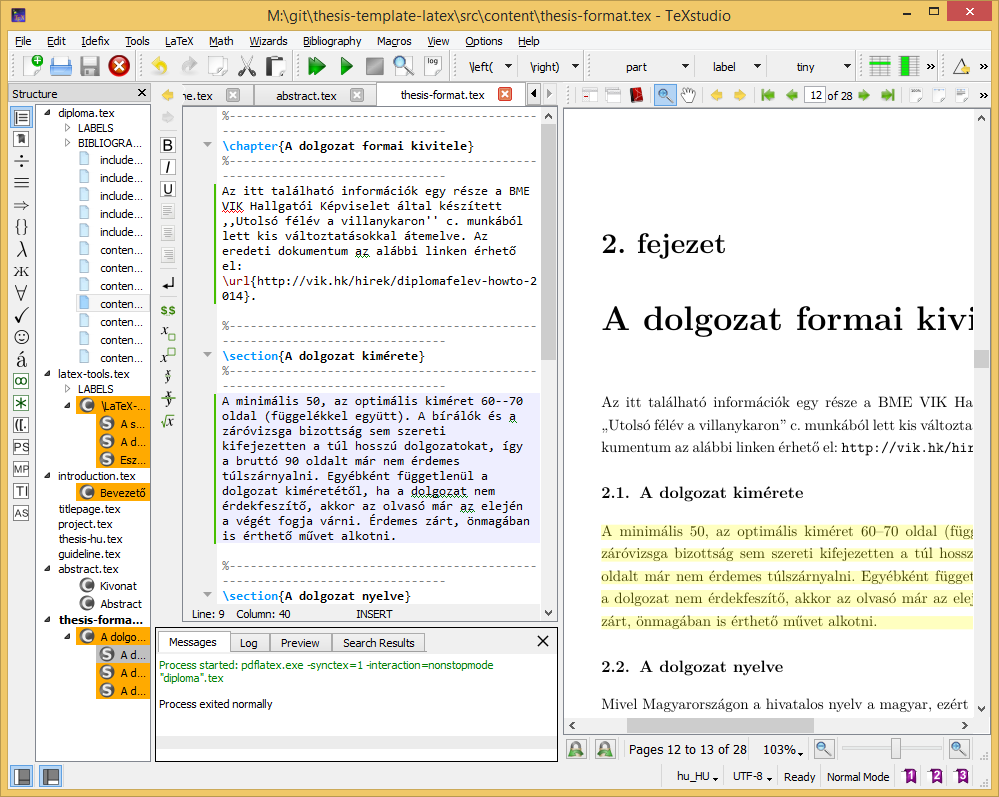
\includegraphics[width=150mm, keepaspectratio]{figures/TeXstudio.png}
\caption{A TeXstudio \LaTeX-szerkesztő.}
\label{fig:TeXstudio}
\end{figure}

A TeXstudio telepítése után érdemes még letölteni a magyar nyelvű helyesírásellenőrző-szótárakat hozzá. A TeXstudio az OpenOffice-hoz használatos formátumot tudja kezelni. A TeXstudio beállításainál a \verb+General+ fülön a \verb+Dictionaries+ résznél tudjuk megadni, hogy melyik szótárat használja.

Egy másik használható Windows alapú szerkesztőprogram a LEd\footnote{A LEd hivatalos oldala: \url{http://www.latexeditor.org/}} (LaTeX Editor), a TeXstudio azonban stabilabb, gyorsabb, és jobban használható.

%----------------------------------------------------------------------------
\section{A dokumentum lefordítása Windows alatt}
%----------------------------------------------------------------------------
A TeXstudio és a LEd kizárólag szerkesztőprogram (bár az utóbbiban DVI-nézegető is van), így a dokumentum fordításához szükséges eszközöket nem tartalmazza. Windows alatt alapvetően két lehetőség közül érdemes választani: MiKTeX (\url{http://miktex.org/}) és TeX Live (\url{http://www.tug.org/texlive/}) programcsomag. Az utóbbi működik Mac OS X, GNU/Linux alatt és Unix-származékokon is. A MiKTeX egy alapcsomag telepítése után mindig letölti a használt funkciókhoz szükséges, de lokálisan hiányzó \TeX-csomagokat, míg a TeX Live DVD ISO verzóban férhető hozzá. Ez a dokumentum TeX Live 2008 programcsomag segítségével fordult, amelynek DVD ISO verziója a megadott oldalról letölthető. A sablon lefordításához a disztribúcióban szereplő \verb+magyar.ldf+ fájlt a \verb+http://www.math.bme.hu/latex/+ változatra kell cserélni, vagy az utóbbi változatot be kell másolni a projekt-könyvtárba (ahogy ezt meg is tettük a sablonban) különben anomáliák tapasztalhatók a dokumentumban (pl. az ábra- és táblázat-aláírások formátuma nem a beállított lesz, vagy bizonyos oldalakon megjelenik alapértelmezésben egy fejléc). A TeX Live 2008-at még nem kell külön telepíteni a gépre, elegendő DVD-ről (vagy az ISO fájlból közvetlenül, pl. DaemonTools-szal) használni.

Ha a MiKTeX csomagot használjuk, akkor parancssorból a következő módon tudjuk újrafordítani a teljes dokumentumot:

\begin{lstlisting}[language=bash,frame=single,float=!ht]
$ texify -p thesis.tex
\end{lstlisting}

A \verb+texify+ parancs a MiKTex programcsomag \verb+miktex/bin+ alkönyvtárában található. A parancs gondoskodik arról, hogy a szükséges lépéseket (fordítás, hivatkozások generálása stb.) a megfelelő sorrendben elvégezze. A \verb+-p+ kapcsoló hatására PDF-et generál. A fordítást és az ideiglenes fájlok törlését elvégezhetjük a sablonhoz mellékelt \verb+manual_build.bat+ szkript segítségével is.

A \TeX-eszközöket tartalmazó programcsomag binárisainak elérési útját gyakran be kell állítani a szerkesztőprogramban, például TeXstudio esetén legegyszerűbben az \verb+Options / Configure TeXstudio... / Commands+ menüponttal előhívott dialógusablakban tehetjük ezt meg.

A PDF-\LaTeX~használata esetén a generált dokumentum közvetlenül PDF-formátumban áll rendelkezésre. Amennyiben a PDF-fájl egy PDF-nézőben (pl. Adobe Acrobat Reader vagy Foxit PDF Reader) meg van nyitva, akkor a fájlleírót a PDF-néző program tipikusan lefoglalja. Ilyen esetben a dokumentum újrafordítása hibaüzenettel kilép. Ha bezárjuk és újra megnyitjuk a PDF dokumentumot, akkor pedig a PDF-nézők többsége az első oldalon nyitja meg a dokumentumot, nem a legutóbb olvasott oldalon. Ezzel szemben például az egyszerű és ingyenes \textcolor{blue}{Sumatra PDF} nevű program képes arra, hogy a megnyitott dokumentum megváltozását detektálja, és frissítse a nézetet az aktuális oldal megtartásával.

%----------------------------------------------------------------------------
\section{Eszközök Linuxhoz}
%----------------------------------------------------------------------------
Linux operációs rendszer alatt is rengeteg szerkesztőprogram van, pl. a KDE alapú Kile jól használható. Ez ingyenesen letölthető, vagy éppenséggel az adott Linux-disztribúció eleve tartalmazza, ahogyan a dokumentum fordításához szükséges csomagokat is. Az Ubuntu Linux disztribúciók alatt például legtöbbször a \verb+texlive-*+ csomagok telepítésével használhatók a \LaTeX-eszközök. A jelen sablon fordításához szükséges csomagok (kb. 0,5 GB) az alábbi paranccsal telepíthetők:

\begin{lstlisting}[language=bash,morekeywords={sudo,apt\-get},alsoletter={-},breaklines=true]
$ sudo apt-get install texlive-latex-extra texlive-fonts-extra texlive-fonts-recommended texlive-xetex texlive-science
\end{lstlisting}

Amennyiben egy újabb csomag hozzáadása után hiányzó fájlra utaló hibát kapunk a fordítótól, telepítenünk kell az azt tartalmazó TeX Live csomagot. Ha pl. a \verb+bibentry+ csomagot szeretnénk használni, futtassuk az alábbi parancsot:

\begin{lstlisting}[language=bash,morekeywords={apt\-cache},alsoletter={-},breaklines=true]
$ apt-cache search bibentry
texlive-luatex - TeX Live: LuaTeX packages
\end{lstlisting}

Majd telepítsük fel a megfelelő TeX Live csomagot, jelen esetben a `texlive-lualatex`-et. (Egy LaTeX csomag több TeX Live csomagban is szerepelhet.)

Ha gyakran szerkesztünk más \LaTeX dokumentumokat is, kényelmes és biztos megoldás a teljes TeX Live disztribúció telepítése, ez azonban kb. 4 GB helyet igényel.

\begin{lstlisting}[language=bash,morekeywords={sudo,apt\-get},alsoletter={-},breaklines=true]
sudo apt-get install texlive-full
\end{lstlisting}

%----------------------------------------------------------------------------
\chapter{A dolgozat formai kivitele}
%----------------------------------------------------------------------------
Az itt található információk egy része a BME VIK Hallgatói Képviselet által készített ,,Utolsó félév a villanykaron'' c. munkából lett kis változtatásokkal átemelve. Az eredeti dokumentum az alábbi linken érhető el: \url{http://vik.hk/hirek/diplomafelev-howto-2015}.

%----------------------------------------------------------------------------
\section{A dolgozat kimérete}
%----------------------------------------------------------------------------
Szakdolgozat esetében minimum 30, 45 körüli ajánlott oldalszám lehet az iránymutató. De mindenképp érdemes rákérdezni a konzulensnél is az elvárásokra, mert tanszékenként változóak lehetnek az elvárások.

Mesterképzésen a Diplomatervezés 1 esetében a beszámoló még inkább az Önálló laboratóriumi beszámolókhoz hasonlít, tanszékenként eltérő formai követelményekkel, -- egy legalább 30 oldal körüli dolgozat az elvárt -- és az elmúlt fél éves munkáról szól. De egyben célszerű, ha ez a végleges diplomaterv alapja is. (A végleges 60-90 oldal körülbelül a hasznos részre nézve)


%----------------------------------------------------------------------------
\section{A dolgozat nyelve}
%----------------------------------------------------------------------------
Mivel Magyarországon a hivatalos nyelv a magyar, ezért alapértelmezésben magyarul kell megírni a dolgozatot. Aki külföldi posztgraduális képzésben akar részt venni, nemzetközi szintű tudományos kutatást szeretne végezni, vagy multinacionális cégnél akar elhelyezkedni, annak célszerű angolul megírnia diplomadolgozatát. Mielőtt a hallgató az angol nyelvű verzió mellett dönt, erősen ajánlott mérlegelni, hogy ez mennyi többletmunkát fog a hallgatónak jelenteni fogalmazás és nyelvhelyesség terén, valamint -- nem utolsó sorban -- hogy ez mennyi többletmunkát fog jelenteni a konzulens illetve bíráló számára. Egy nehezen olvasható, netalán érthetetlen szöveg teher minden játékos számára.

%----------------------------------------------------------------------------
\section{A dokumentum nyomdatechnikai kivitele}
%----------------------------------------------------------------------------
A dolgozatot A4-es fehér lapra nyomtatva, 2,5 centiméteres margóval (+1~cm kötésbeni), 11--12 pontos betűmérettel, talpas betűtípussal és másfeles sorközzel célszerű elkészíteni.

Annak érdekében, hogy a dolgozat külsőleg is igényes munka benyomását keltse, érdemes figyelni az alapvető tipográfiai szabályok betartására~\cite{Jeney}.

% !TeX spellcheck = hu_HU
% !TeX encoding = UTF-8
% !TeX program = xelatex
%----------------------------------------------------------------------------
\chapter{A \LaTeX-sablon használata}
%----------------------------------------------------------------------------

Ebben a fejezetben röviden, implicit módon bemutatjuk a sablon használatának módját, ami azt jelenti, hogy sablon használata ennek a dokumentumnak a forráskódját tanulmányozva válik teljesen világossá. Amennyiben a szoftver-keretrendszer telepítve van, a sablon alkalmazása és a dolgozat szerkesztése \LaTeX-ben a sablon segítségével tapasztalataink szerint jóval hatékonyabb, mint egy WYSWYG (\emph{What You See is What You Get}) típusú szövegszerkesztő esetén (pl. Microsoft Word, OpenOffice).

%----------------------------------------------------------------------------
\section{Címkék és hivatkozások}
%----------------------------------------------------------------------------
A \LaTeX~dokumentumban címkéket (\verb+\label+) rendelhetünk ábrákhoz, táblázatokhoz, fejezetekhez, listákhoz, képletekhez stb. Ezekre a dokumentum bármely részében hivatkozhatunk, a hivatkozások automatikusan feloldásra kerülnek.

A sablonban makrókat definiáltunk a hivatkozások megkönnyítéséhez. Ennek megfelelően minden ábra (\emph{figure}) címkéje \verb+fig:+ kulcsszóval kezdődik, míg minden táblázat (\emph{table}), képlet (\emph{equation}), fejezet (\emph{section}) és lista (\emph{listing}) rendre a \verb+tab:+, \verb+eq:+, \verb+sec:+ és \verb+lst:+ kulcsszóval kezdődik, és a kulcsszavak után tetszőlegesen választott címke használható. Ha ezt a konvenciót betartjuk, akkor az előbbi objektumok számára rendre a \verb+\figref+, \verb+\tabref+, \verb+\eqref+, \verb+\sectref+ és \verb+\listref+ makrókkal hivatkozhatunk. A makrók paramétere a címke, amelyre hivatkozunk (a kulcsszó nélkül). Az összes említett hivatkozástípus, beleértve az \verb+\url+ kulcsszóval bevezetett web-hivatkozásokat is a  \verb+hyperref+\footnote{Segítségével a dokumentumban megjelenő hivatkozások nem csak dinamikussá válnak, de színezhetők is, bővebbet erről a csomag dokumentációjában találunk. Ez egyúttal egy példa lábjegyzet írására.} csomagnak köszönhetően aktívak a legtöbb PDF-nézegetőben, rájuk kattintva a dokumentum megfelelő oldalára ugrik a PDF-néző vagy a megfelelő linket megnyitja az alapértelmezett böngészővel. A \verb+hyperref+ csomag a kimeneti PDF-dokumentumba könyvjelzőket is készít a tartalomjegyzékből. Ez egy szintén aktív tartalomjegyzék, amelynek elemeire kattintva a nézegető behozza a kiválasztott fejezetet.

%----------------------------------------------------------------------------
\section{Ábrák és táblázatok}
%----------------------------------------------------------------------------
Használjunk vektorgrafikus ábrákat, ha van rá módunk. PDFLaTeX használata esetén PDF formátumú ábrákat lehet beilleszteni könnyen, az EPS (PostScript) vektorgrafikus képformátum beillesztését a PDFLaTeX közvetlenül nem támogatja (de lehet konvertálni, lásd később). Ha vektorgrafikus formában nem áll rendelkezésünkre az ábra, akkor a  veszteségmentes PNG, valamint a veszteséges JPEG formátumban érdemes elmenteni.  Figyeljünk arra, hogy ilyenkor a képek felbontása elég nagy legyen ahhoz, hogy nyomtatásban is megfelelő minőséget nyújtson (legalább 300 dpi javasolt). A dokumentumban felhasznált képfájlokat a dokumentum forrása mellett érdemes tartani, archiválni, mivel ezek hiányában a dokumentum nem fordul újra. Ha lehet, a vektorgrafikus képeket vektorgrafikus formátumban is érdemes elmenteni az újrafelhasználhatóság (az átszerkeszthetőség) érdekében.

Kapcsolási rajzok legtöbbször kimásolhatók egy vektorgrafikus programba (pl. CorelDraw) és onnan nagyobb felbontással raszterizálva kimenthatők PNG formátumban. Ugyanakkor kiváló ábrák készíthetők Microsoft Visio vagy hasonló program használatával is: Visio-ból az ábrák közvetlenül PDF-be is menthetők.

Lehetőségeink Matlab ábrák esetén:
\begin{itemize}
	\item Képernyőlopás (\emph{screenshot}) is elfogadható minőségű lehet a dokumentumban, de általában jobb felbontást is el lehet érni más módszerrel.
	\item A Matlab ábrát a \verb+File/Save As+ opcióval lementhetjük PNG formátumban (ugyanaz itt is érvényes, mint korábban, ezért nem javasoljuk).
	\item A Matlab ábrát az \verb+Edit/Copy figure+ opcióval kimásolhatjuk egy vektorgrafikus programba is és onnan nagyobb felbontással raszterizálva kimenthatjük PNG formátumban (nem javasolt).
	\item Javasolt megoldás: az ábrát a \verb+File/Save As+ opcióval EPS \emph{vektorgrafikus} formátumban elmentjük, PDF-be konvertálva beillesztjük a dolgozatba.
\end{itemize}
Az EPS kép az \verb+epstopdf+ programmal\footnote{a korábban említett \LaTeX-disztribúciókban megtalálható} konvertálható PDF formátumba. Célszerű egy batch-fájlt készíteni az összes EPS ábra lefordítására az alábbi módon (ez Windows alatt működik).
\begin{lstlisting}[language=]
@echo off
for %%j in (*.eps) do (
  echo converting file "%%j"
  epstopdf "%%j"
)
echo done .
\end{lstlisting}

Egy ilyen parancsfájlt (\verb+convert.cmd+) elhelyeztük a sablon \verb+figures\eps+ könyvtárába, így a felhasználónak csak annyi a dolga, hogy a \verb+figures\eps+ könyvtárba kimenti az EPS formátumú vektorgrafikus képet, majd lefuttatja a \verb+convert.cmd+ parancsfájlt, ami PDF-be konvertálja az EPS fájlt.

Ezek után a PDF-ábrát ugyanúgy lehet a dokumentumba beilleszteni, mint a PNG-t vagy a JPEG-et. A megoldás előnye, hogy a lefordított dokumentumban is vektorgrafikusan tárolódik az ábra, így a mérete jóval kisebb, mintha raszterizáltuk volna beillesztés előtt. Ez a módszer minden -- az EPS formátumot ismerő -- vektorgrafikus program (pl. CorelDraw) esetén is használható.

A képek beillesztésére \az+\refstruc{sec:LatexTools}ben mutattunk be példát (\refstruc{fig:TeXstudio}). Az előző mondatban egyúttal az automatikusan feloldódó ábrahivatkozásra is láthatunk példát. Több képfájlt is beilleszthetünk egyetlen ábrába. Az egyes képek közötti horizontális és vertikális margót metrikusan szabályozhatjuk (\refstruc{fig:HVSpaces}). Az ábrák elhelyezését számtalan tipográfiai szabály egyidejű teljesítésével a fordító maga végzi, a dokumentum írója csak preferenciáit jelezheti a fordító felé (olykor ez bosszúságot is okozhat, ilyenkor pl. a kép méretével lehet játszani).

\begin{figure}[!ht]
	\centering
	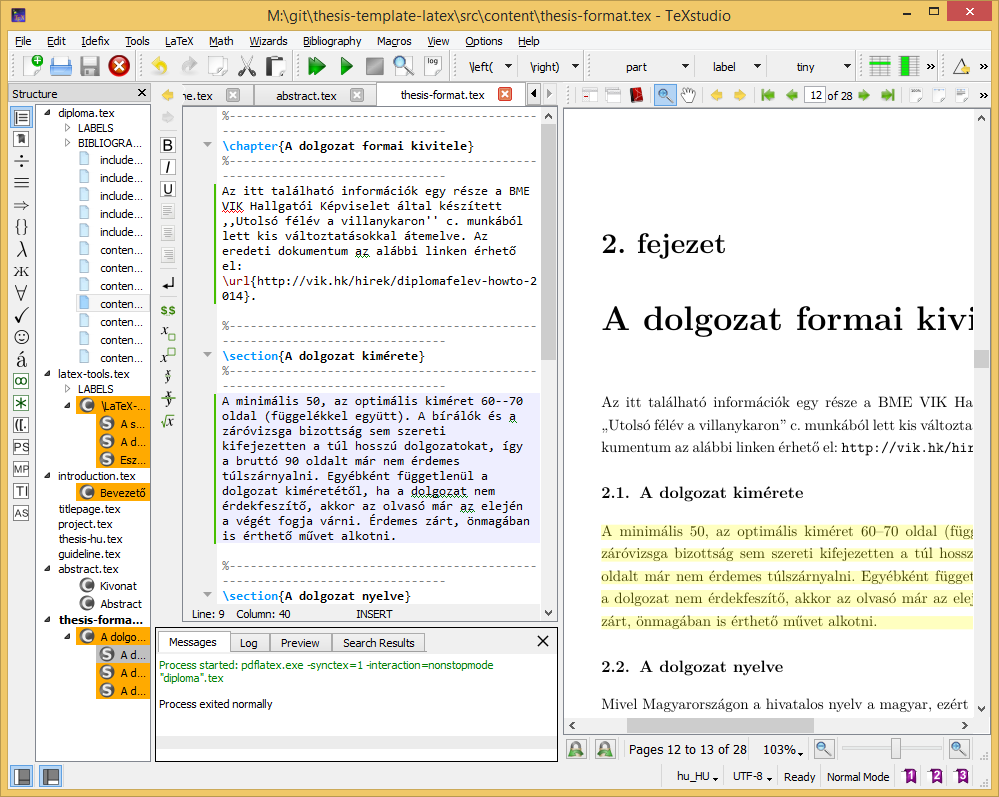
\includegraphics[width=67mm, keepaspectratio]{figures/TeXstudio.png}\hspace{1cm}
	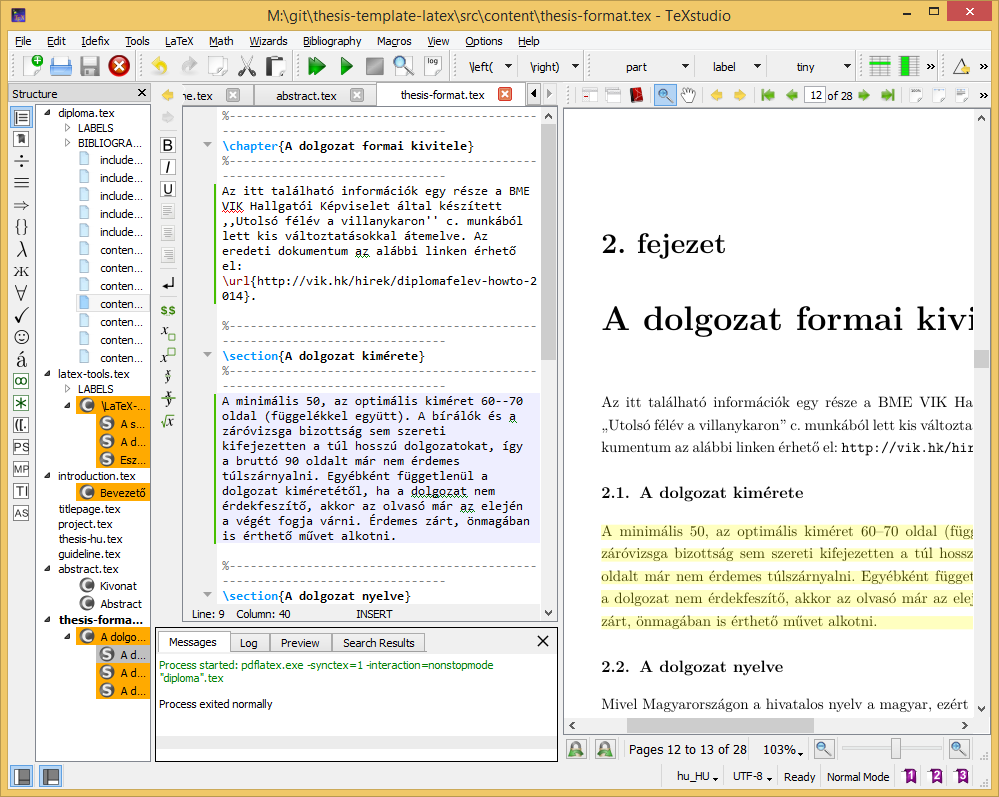
\includegraphics[width=67mm, keepaspectratio]{figures/TeXstudio.png}\\\vspace{5mm}
	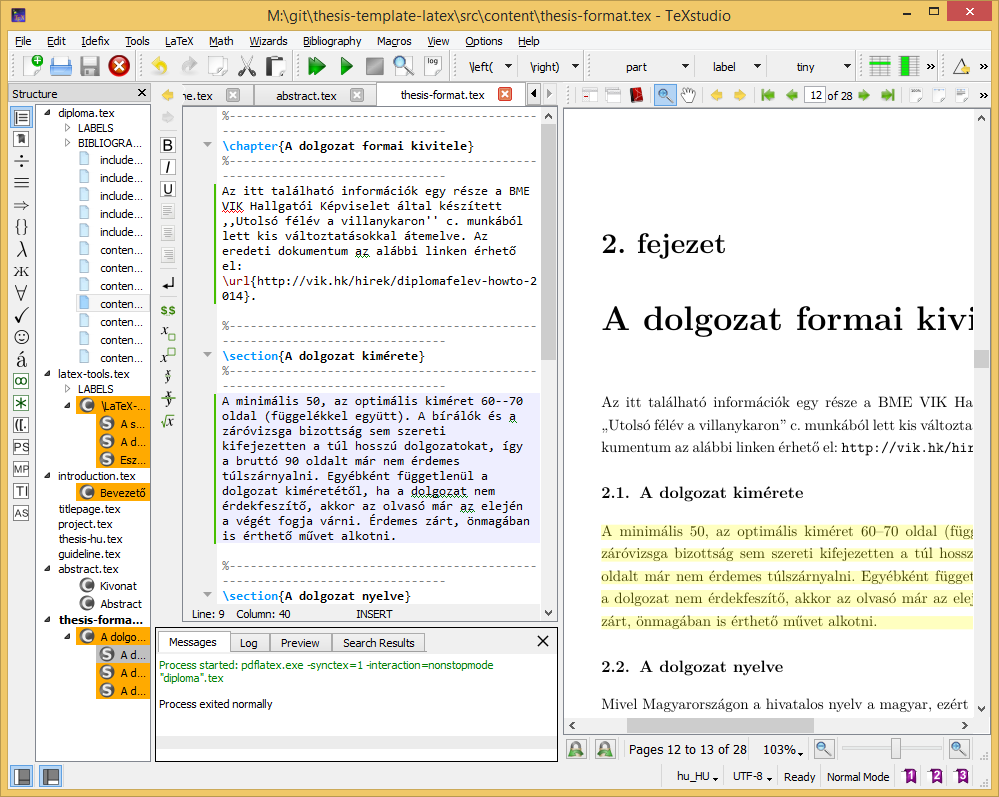
\includegraphics[width=67mm, keepaspectratio]{figures/TeXstudio.png}\hspace{1cm}
	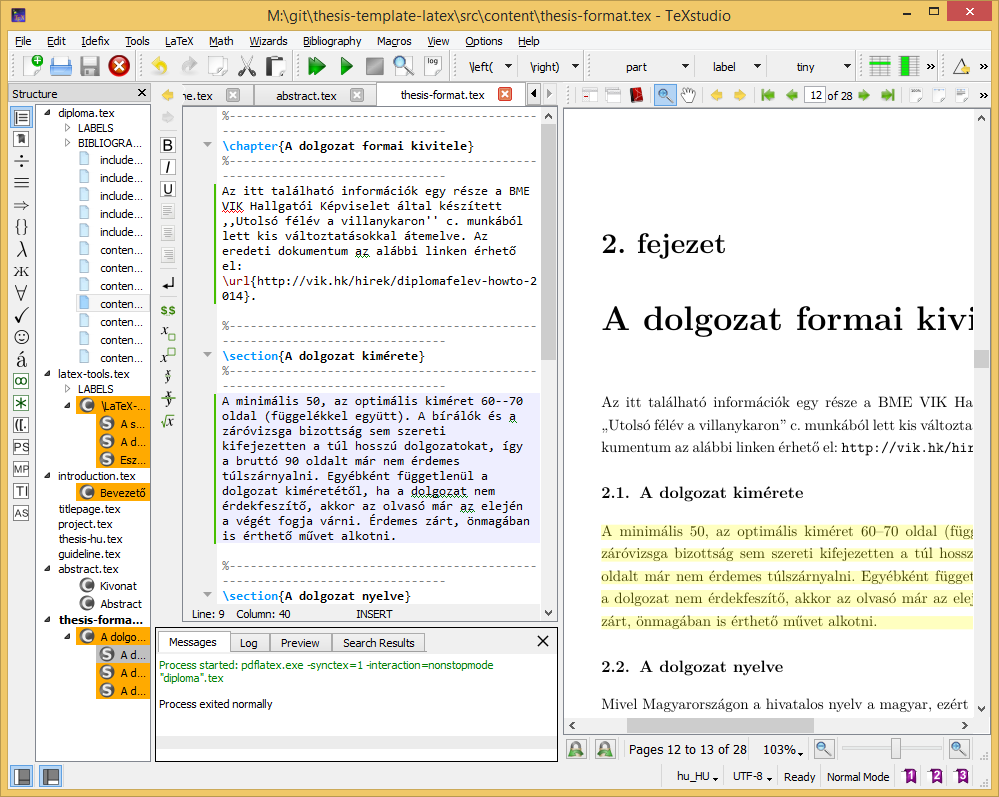
\includegraphics[width=67mm, keepaspectratio]{figures/TeXstudio.png}
	\caption{Több képfájl beillesztése esetén térközöket is érdemes használni.}
	\label{fig:HVSpaces}
\end{figure}

A táblázatok használatára \aref{tab:TabularExample}~táblázat mutat példát. A táblázatok formázásához hasznos tanácsokat találunk a \verb+booktabs+ csomag dokumentációjában.

\begin{table}[ht]
	\footnotesize
	\centering
	\begin{tabular}{ l c c }
		\toprule
		Órajel & Frekvencia & Cél pin \\
		\midrule
		CLKA & 100 MHz & FPGA CLK0\\
		CLKB & 48 MHz  & FPGA CLK1\\
		CLKC & 20 MHz  & Processzor\\
		CLKD & 25 MHz  & Ethernet chip \\
		CLKE & 72 MHz  & FPGA CLK2\\
		XBUF & 20 MHz  & FPGA CLK3\\
		\bottomrule
	\end{tabular}
	\caption{Az órajel-generátor chip órajel-kimenetei.}
	\label{tab:TabularExample}
\end{table}


%----------------------------------------------------------------------------
\section{Felsorolások és listák}
%----------------------------------------------------------------------------
Számozatlan felsorolásra mutat példát a jelenlegi bekezdés:
\begin{itemize}
	\item \emph{első bajusz:} ide lehetne írni az első elem kifejését,
	\item \emph{második bajusz:} ide lehetne írni a második elem kifejését,
	\item \emph{ez meg egy szakáll:} ide lehetne írni a harmadik elem kifejését.
\end{itemize}

Számozott felsorolást is készíthetünk az alábbi módon:
\begin{enumerate}
	\item \emph{első bajusz:} ide lehetne írni az első elem kifejését, és ez a kifejtés így néz ki, ha több sorosra sikeredik,
	\item \emph{második bajusz:} ide lehetne írni a második elem kifejését,
	\item \emph{ez meg egy szakáll:} ide lehetne írni a harmadik elem kifejését.
\end{enumerate}
A felsorolásokban sorok végén vessző, az utolsó sor végén pedig pont a szokásos írásjel. Ez alól kivételt képezhet, ha az egyes elemek több teljes mondatot tartalmaznak.

Listákban a dolgozat szövegétől elkülönítendő kódrészleteket, programsorokat, pszeudo-kódokat jeleníthetünk meg (\ref{lst:Example}.~kódrészlet).
\begin{lstlisting}[language=tex,caption=A fenti számozott felsorolás \LaTeX-forráskódja,label=lst:Example]
\begin{enumerate}
	\item \emph{els(*@ő@*) bajusz:} ide lehetne írni az els(*@ő@*) elem kifejését,
	és ez a kifejtés így néz ki, ha több sorosra sikeredik,
	\item \emph{második bajusz:} ide lehetne írni a második elem kifejését,
	\item \emph{ez meg egy szakáll:} ide lehetne írni a harmadik elem kifejését.
\end{enumerate}
\end{lstlisting}
A lista keretét, háttérszínét, egész stílusát megválaszthatjuk. Ráadásul különféle programnyelveket és a nyelveken belül kulcsszavakat is definiálhatunk, ha szükséges. Erről bővebbet a \verb+listings+ csomag hivatalos leírásában találhatunk.

%----------------------------------------------------------------------------
\section{Képletek}
%----------------------------------------------------------------------------
Ha egy formula nem túlságosan hosszú, és nem akarjuk hivatkozni a szövegből, mint például a $e^{i\pi}+1=0$ képlet, \emph{szövegközi képletként} szokás leírni. Csak, hogy másik példát is lássunk, az $U_i=-d\Phi/dt$ Faraday-törvény a $\rot E=-\frac{dB}{dt}$ differenciális alakban adott Maxwell-egyenlet felületre vett integráljából vezethető le. Látható, hogy a \LaTeX-fordító a sorközöket betartja, így a szöveg szedése esztétikus marad szövegközi képletek használata esetén is.

Képletek esetén az általános konvenció, hogy a kisbetűk skalárt, a kis félkövér betűk ($\mathbf{v}$) oszlopvektort -- és ennek megfelelően $\mathbf{v}^T$ sorvektort -- a kapitális félkövér betűk ($\mathbf{V}$) mátrixot jelölnek. Ha ettől el szeretnénk térni, akkor az alkalmazni kívánt jelölésmódot célszerű külön alfejezetben definiálni. Ennek megfelelően, amennyiben $\mathbf{y}$ jelöli a mérések vektorát, $\mathbf{\vartheta}$ a paraméterek vektorát és $\hat{\mathbf{y}}=\mathbf{X}\vartheta$ a paraméterekben lineáris modellt, akkor a \emph{Least-Squares} értelemben optimális paraméterbecslő $\hat{\mathbf{\vartheta}}_{LS}=(\mathbf{X}^T\mathbf{X})^{-1}\mathbf{X}^T\mathbf{y}$ lesz.

Emellett kiemelt, sorszámozott képleteket is megadhatunk, ennél az \verb+equation+ és a \verb+eqnarray+ környezetek helyett a korszerűbb \verb+align+ környezet alkalmazását javasoljuk (több okból, különféle problémák elkerülése végett, amelyekre most nem térünk ki). Tehát
\begin{align}
\dot{\mathbf{x}}&=\mathbf{A}\mathbf{x}+\mathbf{B}\mathbf{u},\\
\mathbf{y}&=\mathbf{C}\mathbf{x},
\end{align}
ahol $\mathbf{x}$ az állapotvektor, $\mathbf{y}$ a mérések vektora és $\mathbf{A}$, $\mathbf{B}$ és $\mathbf{C}$ a rendszert leíró paramétermátrixok. Figyeljük meg, hogy a két egyenletben az egyenlőségjelek egymáshoz igazítva jelennek meg, mivel a mindkettőt az \& karakter előzi meg a kódban. Lehetőség van számozatlan kiemelt képlet használatára is, például
\begin{align}
\dot{\mathbf{x}}&=\mathbf{A}\mathbf{x}+\mathbf{B}\mathbf{u},\nonumber\\
\mathbf{y}&=\mathbf{C}\mathbf{x}\nonumber.
\end{align}
Mátrixok felírására az $\mathbf{A}\mathbf{x}=\mathbf{b}$ inhomogén lineáris egyenlet részletes kifejtésével mutatunk példát:
\begin{align}
\begin{bmatrix}
a_{11} & a_{12} & \dots & a_{1n}\\
a_{21} & a_{22} & \dots & a_{2n}\\
\vdots & \vdots & \ddots & \vdots\\
a_{m1} & a_{m2} & \dots & a_{mn}
\end{bmatrix}
\begin{pmatrix}x_1\\x_2\\\vdots\\x_n\end{pmatrix}=
\begin{pmatrix}b_1\\b_2\\\vdots\\b_m\end{pmatrix}.
\end{align}
A \verb+\frac+ utasítás hatékonyságát egy általános másodfokú tag átviteli függvényén keresztül mutatjuk be, azaz
\begin{align}
W(s)=\frac{A}{1+2T\xi s+s^2T^2}.
\end{align}
A matematikai mód minden szimbólumának és képességének a bemutatására természetesen itt nincs lehetőség, de gyors referenciaként hatékonyan használhatók a következő linkek:\\
\indent\url{http://www.artofproblemsolving.com/LaTeX/AoPS_L_GuideSym.php},\\
\indent\url{http://www.ctan.org/tex-archive/info/symbols/comprehensive/symbols-a4.pdf},\\
\indent\url{ftp://ftp.ams.org/pub/tex/doc/amsmath/short-math-guide.pdf}.\\
Ez pedig itt egy magyarázat, hogy miért érdemes \verb+align+ környezetet használni:\\
\indent\url{http://texblog.net/latex-archive/maths/eqnarray-align-environment/}.

%----------------------------------------------------------------------------
\section{Irodalmi hivatkozások}
\label{sec:HowtoReference}
%----------------------------------------------------------------------------
Egy \LaTeX~dokumentumban az irodalmi hivatkozások definíciójának két módja van. Az egyik a \verb+\thebibliograhy+ környezet használata a dokumentum végén, az \verb+\end{document}+ lezárás előtt.
\begin{lstlisting}[language=tex]
\begin{thebibliography}{9}

\bibitem{Lamport94} Leslie Lamport, \emph{\LaTeX: A Document Preparation System}.
Addison Wesley, Massachusetts, 2nd Edition, 1994.

\end{thebibliography}
\end{lstlisting}

Ezek után a dokumentumban a \verb+\cite{Lamport94}+ utasítással hivatkozhatunk a forrásra. A fenti megadás viszonylag kötetlen, a szerző maga formázza az irodalomjegyzéket (ami gyakran inkonzisztens eredményhez vezet).

Egy sokkal professzionálisabb módszer a BiB\TeX{} használata, ezért ez a sablon is ezt támogatja. Ebben az esetben egy külön szöveges adatbázisban definiáljuk a forrásmunkákat, és egy külön stílusfájl határozza meg az irodalomjegyzék kinézetét. Ez, összhangban azzal, hogy külön formátumkonvenció határozza meg a folyóirat-, a könyv-, a konferenciacikk- stb. hivatkozások kinézetét az irodalomjegyzékben (a sablon használata esetén ezzel nem is kell foglalkoznia a hallgatónak, de az eredményt célszerű ellenőrizni). felhasznált hivatkozások adatbázisa egy \verb+.bib+ kiterjesztésű szöveges fájl, amelynek szerkezetét a \Aref{lst:Bibtex} kódrészlet demonstrálja. A forrásmunkák bevitelekor a sor végi vesszők külön figyelmet igényelnek, mert hiányuk a BiB\TeX-fordító hibaüzenetét eredményezi. A forrásmunkákat típus szerinti kulcsszó vezeti be (\verb+@book+ könyv, \verb+@inproceedings+ konferenciakiadványban megjelent cikk, \verb+@article+ folyóiratban megjelent cikk, \verb+@techreport+ valamelyik egyetem gondozásában megjelent műszaki tanulmány, \verb+@manual+ műszaki dokumentáció esetén stb.). Nemcsak a megjelenés stílusa, de a kötelezően megadandó mezők is típusról-típusra változnak. Egy jól használható referencia a \url{http://en.wikipedia.org/wiki/BibTeX} oldalon található.

\begin{lstlisting}[caption=Példa szöveges irodalomjegyzék-adatbázisra Bib\TeX{} használata esetén.,label=lst:Bibtex]
@book{Wettl04,
  author    = {Ferenc Wettl and Gyula Mayer and Péter Szabó},
  publisher = {Panem Könyvkiadó},
  title     = {\LaTeX~kézikönyv},
  year      = {2004},
}

@article{Candy86,
  author       = {James C. Candy},
  journaltitle = {{IEEE} Trans.\ on Communications},
  month        = {01},
  note         = {\doi{10.1109/TCOM.1986.1096432}},
  number       = {1},
  pages        = {72--76},
  title        = {Decimation for Sigma Delta Modulation},
  volume       = {34},
  year         = {1986},
}

@inproceedings{Lee87,
  author    = {Wai L. Lee and Charles G. Sodini},
  booktitle = {Proc.\ of the IEEE International Symposium on Circuits and Systems},
  location  = {Philadelphia, PA, USA},
  month     = {05~4--7},
  pages     = {459--462},
  title     = {A Topology for Higher Order Interpolative Coders},
  vol       = {2},
  year      = {1987},
}

@thesis{KissPhD,
  author      = {Peter Kiss},
  institution = {Technical University of Timi\c{s}oara, Romania},
  month       = {04},
  title       = {Adaptive Digital Compensation of Analog Circuit Imperfections for Cascaded Delta-Sigma Analog-to-Digital Converters},
  type        = {phdthesis},
  year        = {2000},
}

@manual{Schreier00,
  author       = {Richard Schreier},
  month        = {01},
  note         = {\url{http://www.mathworks.com/matlabcentral/fileexchange/}},
  organization = {Oregon State University},
  title        = {The Delta-Sigma Toolbox v5.2},
  year         = {2000},
}

@misc{DipPortal,
  author       = {{Budapesti Műszaki és Gazdaságtudományi Egyetem Villamosmérnöki és Informatikai Kar}},
  howpublished = {\url{http://diplomaterv.vik.bme.hu/}},
  title        = {Diplomaterv portál (2011. február 26.)},
}

@incollection{Mkrtychev:1997,
  author    = {Mkrtychev, Alexey},
  booktitle = {Logical Foundations of Computer Science},
  doi       = {10.1007/3-540-63045-7_27},
  editor    = {Adian, Sergei and Nerode, Anil},
  isbn      = {978-3-540-63045-6},
  pages     = {266-275},
  publisher = {Springer Berlin Heidelberg},
  series    = {Lecture Notes in Computer Science},
  title     = {Models for the logic of proofs},
  url       = {http://dx.doi.org/10.1007/3-540-63045-7_27},
  volume    = {1234},
  year      = {1997},
}
\end{lstlisting}

A stílusfájl egy \verb+.sty+ kiterjesztésű fájl, de ezzel lényegében nem kell foglalkozni, mert vannak beépített stílusok, amelyek jól használhatók. Ez a sablon a BiB\TeX-et használja, a hozzá tartozó adatbázisfájl a \verb+mybib.bib+ fájl. Megfigyelhető, hogy az irodalomjegyzéket a dokumentum végére (a \verb+\end{document}+ utasítás elé) beillesztett \verb+\bibliography{mybib}+ utasítással hozhatjuk létre, a stílusát pedig ugyanitt a  \verb+\bibliographystyle{plain}+ utasítással adhatjuk meg. Ebben az esetben a \verb+plain+ előre definiált stílust használjuk (a sablonban is ezt állítottuk be). A \verb+plain+ stíluson kívül természetesen számtalan más előre definiált stílus is létezik. Mivel a \verb+.bib+ adatbázisban ezeket megadtuk, a BiB\TeX-fordító is meg tudja különböztetni a szerzőt a címtől és a kiadótól, és ez alapján automatikusan generálódik az irodalomjegyzék a stílusfájl által meghatározott stílusban.

Az egyes forrásmunkákra a szövegből továbbra is a \verb+\cite+ paranccsal tudunk hivatkozni, így \aref{lst:Bibtex}.~kódrészlet esetén a hivatkozások rendre \verb+\cite{Wettl04}+, \verb+\cite{Candy86}+, \verb+\cite{Lee87}+, \verb+\cite{KissPhD}+, \verb+\cite{Schreirer00}+,
\verb+\cite{Mkrtychev:1997}+ és \verb+\cite{DipPortal}+. Az egyes forrásmunkák sorszáma az irodalomjegyzék bővítésekor változhat. Amennyiben az aktuális számhoz illeszkedő névelőt szeretnénk használni, használjuk az \verb+\acite{}+ parancsot.

Az irodalomjegyzékben alapértelmezésben csak azok a forrásmunkák jelennek meg, amelyekre található hivatkozás a szövegben, és ez így alapvetően helyes is, hiszen olyan forrásmunkákat nem illik az irodalomjegyzékbe írni, amelyekre nincs hivatkozás.

Mivel a fordítási folyamat során több lépésben oldódnak fel a szimbólumok, ezért gyakran többször is le kell fordítani a dokumentumot. Ilyenkor ez első 1-2 fordítás esetleg szimbólum-feloldásra vonatkozó figyelmeztető üzenettel zárul. Ha hibaüzenettel zárul bármelyik fordítás, akkor nincs értelme megismételni, hanem a hibát kell megkeresni. A \verb+.bib+ fájl megváltoztatáskor sokszor nincs hatása a változtatásnak azonnal, mivel nem mindig fut újra a BibTeX fordító. Ezért célszerű a változtatás után azt manuálisan is lefuttatni (TeXstudio esetén \verb+Tools/Bibliography+).

Hogy a szövegbe ágyazott hivatkozások kinézetét demonstráljuk, itt most sorban meghivatkozzuk a \cite{Wettl04}, \cite{Candy86}, \cite{Lee87}, \cite{KissPhD}, \cite{Schreier00} és \acite{Mkrtychev:1997}\footnote{Informatikai témában gyakran hivatkozunk cikkeket a Springer LNCS valamely kötetéből, ez a hivatkozás erre mutat egy helyes példát.} forrásmunkát, valamint \acite{DipPortal} weboldalt.

Megjegyzendő, hogy az ékezetes magyar betűket is tartalmazó \verb+.bib+ fájl az \verb+inputenc+ csomaggal betöltött \verb+latin2+ betűkészlet miatt fordítható. Ugyanez a \verb+.bib+ fájl hibaüzenettel fordul egy olyan dokumentumban, ami nem tartalmazza a \verb+\usepackage[latin2]{inputenc}+ sort. Speciális igény esetén az irodalmi adatbázis általánosabb érvényűvé tehető, ha az ékezetes betűket speciális latex karakterekkel helyettesítjük a \verb+.bib+ fájlban, pl. á helyett \verb+\'{a}+-t vagy ő helyett \verb+\H{o}+-t írunk.

Irodalomhivatkozásokat célszerű először olyan szolgáltatásokban keresni, ahol jó minőségű bejegyzések találhatók (pl. ACM Digital Library,\footnote{\url{https://dl.acm.org/}} DBLP,\footnote{\url{http://dblp.uni-trier.de/}} IEEE Xplore,\footnote{\url{http://ieeexplore.ieee.org/}} SpringerLink\footnote{\url{https://link.springer.com/}}) és csak ezek után használni kevésbé válogatott forrásokat (pl. Google Scholar\footnote{\url{http://scholar.google.com/}}). A jó minőségű bejegyzéseket is érdemes megfelelően tisztítani.\footnote{\url{https://github.com/FTSRG/cheat-sheets/wiki/BibTeX-Fixing-entries-from-common-sources}} A sablon angol nyelvű változatában használt \texttt{plainnat} beállítás egyik sajátossága, hogy a cikkhez generált hivatkozás a cikk DOI-ját és URL-jét is tartalmazza, ami gyakran duplikátumhoz vezet -- érdemes tehát a DOI-kat tartalmazó URL mezőket törölni. 

%----------------------------------------------------------------------------
\section{A dolgozat szerkezete és a forrásfájlok}
%----------------------------------------------------------------------------
A diplomatervsablonban a TeX fájlok két alkönyvtárban helyezkednek el. Az \verb+include+ könyvtárban azok szerepelnek, amiket tipikusan nem kell szerkesztenünk, ezek a sablon részei (pl. címoldal). A \verb+content+ alkönyvtárban pedig a saját munkánkat helyezhetjük el. Itt érdemes az egyes fejezeteket külön \TeX{} állományokba rakni.

A diplomatervsablon (a kari irányelvek szerint) az alábbi fő fejezetekből áll:
\begin{enumerate}
	\item 1 oldalas \emph{tájékoztató} a szakdolgozat/diplomaterv szerkezetéről (\verb+include/guideline.tex+), ami a végső dolgozatból törlendő,
	\item \emph{feladatkiírás} (\verb+include/project.tex+), a dolgozat nyomtatott verzójában ennek a helyére kerül a tanszék által kiadott, a tanszékvezető által aláírt feladatkiírás, a dolgozat elektronikus verziójába pedig a feladatkiírás egyáltalán ne kerüljön bele, azt külön tölti fel a tanszék a diplomaterv-honlapra,
	\item \emph{címoldal} (\verb+include/titlepage.tex+),
	\item \emph{tartalomjegyzék} (\verb+thesis.tex+),
	\item a diplomatervező \emph{nyilatkozat}a az önálló munkáról (\verb+include/declaration.tex+),
	\item 1-2 oldalas tartalmi \emph{összefoglaló} magyarul és angolul, illetve elkészíthető még további nyelveken is (\verb+content/abstract.tex+),
	\item \emph{bevezetés}: a feladat értelmezése, a tervezés célja, a feladat indokoltsága, a diplomaterv felépítésének rövid összefoglalása (\verb+content/introduction.tex+),
	\item sorszámmal ellátott \emph{fejezetek}: a feladatkiírás pontosítása és részletes elemzése, előzmények (irodalomkutatás, hasonló alkotások), az ezekből levonható következtetések, a tervezés részletes leírása, a döntési lehetőségek értékelése és a választott megoldások indoklása, a megtervezett műszaki alkotás értékelése, kritikai elemzése, továbbfejlesztési lehetőségek,
	\item esetleges \emph{köszönetnyilvánítás}ok (\verb+content/acknowledgement.tex+),
	\item részletes és pontos \emph{irodalomjegyzék} (ez a sablon esetében automatikusan generálódik a \verb+thesis.tex+ fájlban elhelyezett \verb+\bibliography+ utasítás hatására, \az+\refstruc{sec:HowtoReference}ban leírtak szerint),
	\item \emph{függelékek} (\verb+content/appendices.tex+).
\end{enumerate}

A sablonban a fejezetek a \verb+thesis.tex+ fájlba vannak beillesztve \verb+\include+ utasítások segítségével. Lehetőség van arra, hogy csak az éppen szerkesztés alatt álló \verb+.tex+ fájlt fordítsuk le, ezzel lerövidítve a fordítási folyamatot. Ezt a lehetőséget az alábbi kódrészlet biztosítja a \verb+thesis.tex+ fájlban.
\begin{lstlisting}
\includeonly{
	guideline,%
	project,%
	titlepage,%
	declaration,%
	abstract,%
	introduction,%
	chapter1,%
	chapter2,%
	chapter3,%
	acknowledgement,%
	appendices,%
}
\end{lstlisting}

Ha az alábbi kódrészletben az egyes sorokat a \verb+%+ szimbólummal kikommentezzük, akkor a megfelelő \verb+.tex+ fájl nem fordul le. Az oldalszámok és a tartalomjegyék természetesen csak akkor billennek helyre, ha a teljes dokumentumot lefordítjuk.

%----------------------------------------------------------------------------
\newpage
\section{Alapadatok megadása}
%----------------------------------------------------------------------------
A diplomaterv alapadatait (cím, szerző, konzulens, konzulens titulusa) a \verb+thesis.tex+ fájlban lehet megadni.

%----------------------------------------------------------------------------
\section{Új fejezet írása}
%----------------------------------------------------------------------------
A főfejezetek külön \verb+content+ könyvtárban foglalnak helyet. A sablonhoz 3 fejezet készült. További főfejezeteket úgy hozhatunk létre, ha új \TeX~fájlt készítünk a fejezet számára, és a \verb+thesis.tex+ fájlban, a \verb+\include+ és \verb+\includeonly+ utasítások argumentumába felvesszük az új \verb+.tex+ fájl nevét.


%----------------------------------------------------------------------------
\section{Definíciók, tételek, példák}
%----------------------------------------------------------------------------

\begin{definition}[Fluxuskondenzátor térerőssége]
Lorem ipsum dolor sit amet, consectetur adipiscing elit, sed do eiusmod tempor incididunt ut labore et dolore magna aliqua. Ut enim ad minim veniam, quis nostrud exercitation ullamco laboris nisi ut aliquip ex ea commodo consequat.
\end{definition}

\begin{example}
Példa egy példára. Duis aute irure dolor in reprehenderit in voluptate velit esse cillum dolore eu fugiat nulla pariatur. Excepteur sint occaecat cupidatat non proident, sunt in culpa qui officia deserunt mollit anim id est laborum.
\end{example}

\begin{theorem}[Kovács tétele]
Duis aute irure dolor in reprehenderit in voluptate velit esse cillum dolore eu fugiat nulla pariatur. Excepteur sint occaecat cupidatat non proident, sunt in culpa qui officia deserunt mollit anim id est laborum.
\end{theorem}

\chapter{Használt technológiák kiválasztása}

%----------------------------------------------------------------------------
\section{Frontend}
%----------------------------------------------------------------------------
\subsection{JavaScript keretrendszer}
A frontendhez használt technológia kiválasztásánál két fő szempontot tudunk megkülönböztetni.
Az egyik az egyes backend rendszerek által támogatott, szerveroldalon renderlet, template engine-t használó megoldás, a másik a külön frontend framework használata.
Utóbbi jóval nagyobb szabadságot és funkcionalitást ad a fejlesztő kezébe, és lehetőséget ad a legújabb technikák és könyvtárak használatára.
Emiatt úgy döntöttem, hogy az alkalmazás ezen részét a négy legnépszerűbb keretrendszer (React, Angular, Vue és Svelte) egyikével fogom megvalósítani.
Ezek a keretrendszerek alapvető filozófiában és funkcionalitásban lényegében megyegyeznek, azonban az elérhető 3rd party könyvtárak mennyisége és minősége a React esetében a legnagyobb, emiatt végső soron erre esett a választásom.

\subsection{CSS keretrendszer}
A CSS keretrendszer kiválasztása során két fő irányvonal jött szóba: az ún. atomic CSS, illetve az előre már elkészített komponenseket kínáló könyvtárak.
Míg előbbi lehetővé teszi a teljesen egyedi design írását, utóbbi jóval nagyobb fokú kényelmet és a felület gyorsabb elkészítését teszi lehetővé.
Mivel jelen alkalmazás esetében nem volt szempont egy egyedi design elkészítése, ezért az utóbbi megoldás használata mellett döntöttem.
A kiválasztott framework végül a Chakra UI lett, mely nagy mennyiségű kész, egyszerűen bővíthető és magas fokú accessibility-t kínáló komponensekkel rendelkezik.

%----------------------------------------------------------------------------
\section{Backend}
%----------------------------------------------------------------------------
A backend keretrendszer kiválasztása során a legfontosabb szempont az volt, hogy minél jobban képes legyen integrálódni a frontend keretrendszerhez.
Mindenképpen szerettem volna elkerülni a külön repository használtatát. Ennek fő okai, hogy mind a fejlesztés, mind a deployment jelentősen egyszerűsödik.
A fentiek miatt a lehetőségeim a NodeJS alapú megoldásokra szűkítettem le. Egy népszerű, és általam már kipróbált megoldás az Express keretrendszer, azonban a React világában létezik egy, az igényeimnek méginkább megfelelő framework: a NextJS.
Ez egy React-ra épülő, SSR-t (TODO: lábjegyzet) támogató keretrendszer, amely rendelkezik egy ún. API routes nevű funkcióval.
Ennek segítségével a React alkalmazásunkon belül készíthető egy API réteg, amely a fordítás után szerveroldalon futó függvényekké lesz átalakítva.
Ezzel lényegében megspóroljuk, hogy külön API-t és hozzávaló elérési, illetve deployment környezetet kelljen létrehozni, miközben egy Express-hez hasonló interfészt tudunk használni.
Előnye továbbá, hogy rendkívül egyszerűvé teszi a frontend és a backend közötti kódmegosztást, csökkentve ezzel a duplikációkat és erősítve a type safety-t.

%----------------------------------------------------------------------------
\section{Adatbázis}
%----------------------------------------------------------------------------
Az adatbázis architektúra kiválasztása esetén két fő irányvonal volt a meghatározó: a hagyományos relációs adatbázis (pl. PostgreSQL, MySQL) és a NoSQL megoldások (pl. MongoDB, Google Firestore, AWS DynamoDB).
A technológia kiválasztása során fontos szempont volt az ACID elvek követése, a relációk egyszerű kezelése és a minél nagyobb típusbiztosság elérése a backend kódjában.
Ezeknek a szempontoknak a hagyományos relációs adatbázisok felelnek meg, ezen belül a PostgreSQL-re esett a választásom, mivel ez egy általam már ismert, sok funkciót támogató, inegyenes és nyílt forráskódú megoldás.

%----------------------------------------------------------------------------
\subsection{Az adatbázis elérése}
%----------------------------------------------------------------------------
Miután a backend és adatbázis technológiák és könyvtárak kiválasztásra kerültek, szükséges a kettő közötti kommunikációt biztosító könyvtár meghatározására.
NodeJS környezetben rendkívül nagy választék áll rendelkezésre, ezeket két nagy csoportra lehet bontani: ORM és query builder.
Míg az előbbi megoldás egy erős absztrakciós réteget képez az adatbázis szerkezete és a programkód között, addig a query builder egy, az SQL-hez közelebbi interfészt kínál a felhasználónak.
Ez utóbbi előnye, hogy a felhasználó által írt kód közelebb van a végső soron lefutó SQL-hez, így átláthatóbbak az egyes lekérések végeredményei.
A query builder megoldások közül is kiemelkedik a Prisma, amely egy NodeJS környezetben működő adatbázis kliens, ami a hansúlyt a type safety-re helyezi.
Az adatbázis sémát egy speciális .prisma kiterjesztésű fájlban tudjuk megírni, majd ezt a Prisma migrációs eszközével tudjuk az adatbázisunkba átvezetni. (TODO: lábjegyzet hogy a migráció még csak experimental)
Ezután lehetőségünk van a séma alapján a sémából TypeScript típusokat generálni, melyek használata nagyban megkönnyíti és felgyorsítja a fejlesztés menetét.

\begin{lstlisting}[language=Java, caption=Adatbázis beillesztés TypeORM környezetben]
const user = new User()
user.firstName = "Bob"
user.lastName = "Smith"
user.age = 25
await repository.save(user)
\end{lstlisting}

\begin{lstlisting}[language=Java, caption=Adatbázis beillesztés Prisma segítségével]
const user = await prisma.user.create({
  data: {
    firstName: "Bob",
    lastName: "Smith",
    age: 25
  }
})
\end{lstlisting}

todo: táblázat

                  ORM                     query builder
paradigma         oop                  funkcionális programozás
séma definíció  ts class+dekorátorok         változó
adatelérés     példányosított            query interface, chain-elt függvények
              objektumon keresztül




\section{REST és GraphQL}
Előnyök és hátrányok mindkét esetben, miért rest lett végül (egyszerű, zero-config, ismert, API routes-szal jól integrálódik)

A fentieken túl utolsó lépésként szükséges volt eldönteni a frontend és a backend közötti kommunikáció lebonyolítását (TODO: ezt szebben).
A REST architektúra mellett ugyanis megjelent a GraphQl, ami az eddigi lehetőségekhez képest egy flexibilisebb megoldást kínál az adatok elérésére.
A két technológia előnyeit és hátrányait az alábbi táblázatban foglaltam össze.

TODO: táblázat

A fenti szempontokat figyelembe véve végül a hagyományos REST architektúra alkalmazása mellett döntöttem.

\chapter{Az alkalmazás felépítése}

Az alkalmazás három fő rétege az adatbázis, a backend és a frontend. Az alábbi fejezet ezen három réteg architektúrális
felépítésésről valamint az egyes rétegek összeköttetéséről foglalkozik.

\begin{figure}[!ht]
  \centering
  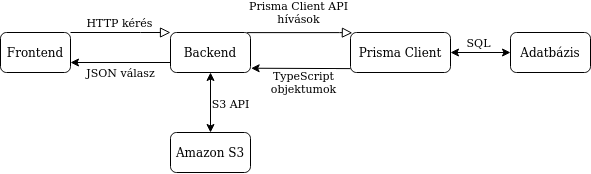
\includegraphics[width=150mm, keepaspectratio]{figures/architecture-diagram.png}
  \caption{Az alkalmazás high-level architektúrája}
  \label{fig:Architecture}
\end{figure}

\section{Adatbázisséma}

Az adatbázisséma tervezéséhez a dbdiagram.io nevű platformfüggetlen, webes ER diagram tervező szoftvert használtam.
Ez egy saját fejlesztésű, DBML nevű DSL nyelvet használ a séma leírására, és lehetővé teszi ennek exportálását különféle formátumokba.

\begin{figure}[!ht]
\centering
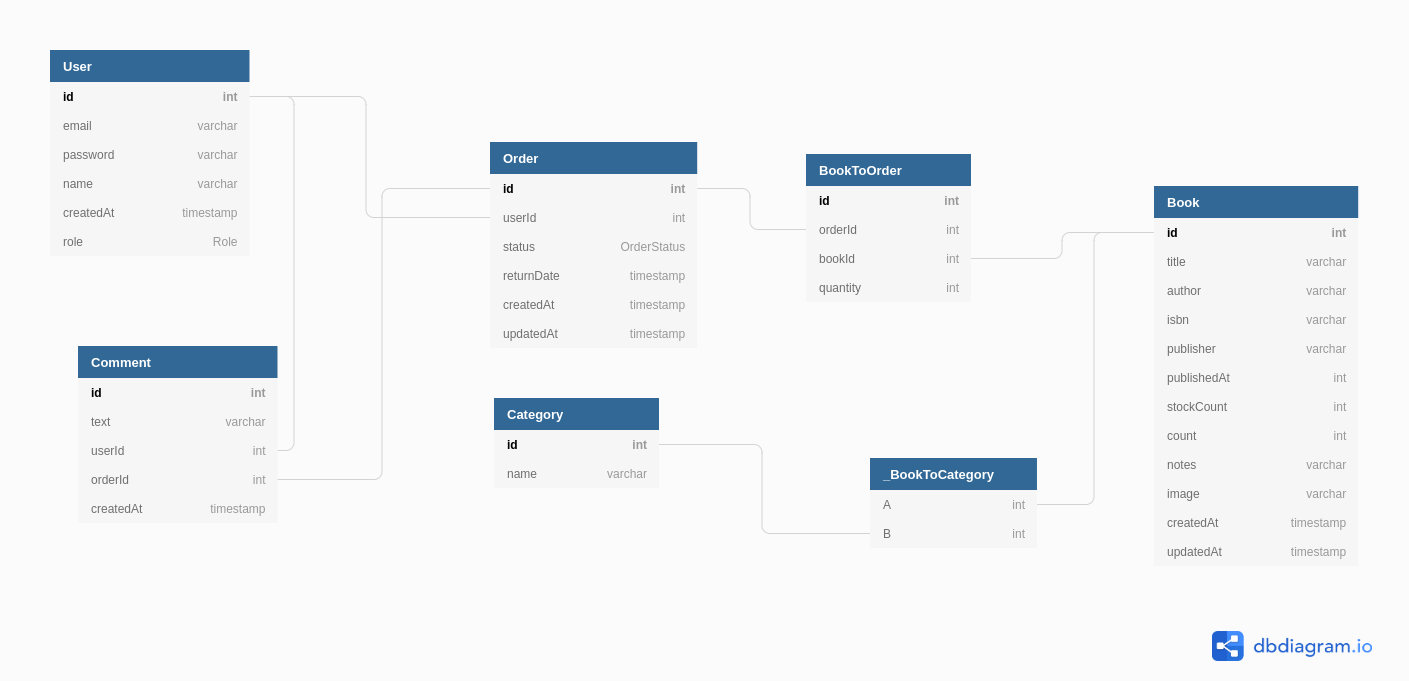
\includegraphics[width=150mm, keepaspectratio]{figures/dbschema.png}
\caption{Az adatbázisséma ER diagramja.}
\label{fig:DBSchema}
\end{figure}

A séma tervezése során a Prisma által használt elnevezési konvenciókat használtam megkönnyítve a két technológia közötti átjárhatóságot.


\section{A backend felépítése}

\subsection{Next.js API routes}

A Next.js keretrendszer a 9-es verzió óta lehetővé teszi szerveroldali kód írását az alkalmazásunkhoz.
Ennek segítségével a \lstinline|pages/api| mappába helyetett fájljaink szolgálnak backendként. Minden ide helyezett fájl
egyben a nevének megfelelő API végpont lesz, tehát például a \lstinline|pages/api/books.ts|-ben lévő kódot a pages/api/books URL-en keresztül tudjuk elérni.

Támogatja továbbá a backend-oldali dinamikus routing-ot, azaz például a \lstinline|pages/api/books/[id].tsx| fájl a \lstinline|pages/api/<id>| URL-nek felel meg, ahol
az \lstinline|id| változót alábbi módon érhetjük el:

\begin{lstlisting}[language=Java, caption=Next.js dinamikus routing]
export default function handler(req, res) {
  const {
    query: { id },
  } = req

  res.end(`Book: ${id}`)
}
\end{lstlisting}

\subsection{next-connect}
Alapesetben a Next.js csak egy egyszerű interface-t biztosít nekünk, amin keresztül elérhetjük a HTTP kérés request és response objektumokat annak kezeléséhez.
Ez azonban nezhézkessé teszi a különböző kérések feldolgozását (pl. GET, POST és PUT), valamint különbőző kódrészletek egyszerű újrafelhasználását.

Ennek kényelmesebbé tételére döntöttem a next-connect könyvtár használata mellett, amellyel a fenti igények könnyedén megvalósíthatóak.
Az alábbi két kódrészletben szeretném bemutatni a főbb különbségeket.

\begin{lstlisting}[language=Java, caption=Default Next.js API routes]
export default function handler(req: NextApiRequest, res: NextApiResponse) {
  if (req.method === 'GET') {
    res.statusCode = 200
    res.setHeader('Content-Type', 'application/json')
    res.end(JSON.stringify({ name: 'John Doe' }))
  } else if (req.method === 'POST') {
    // Process a POST request
  }
}
\end{lstlisting}

\begin{lstlisting}[language=Java, caption=Kérés kezelése next-connect segítségével]
import nextConnect from "next-connect"

const handler = nextConnect<NextApiRequest, NextApiResponse>()

handler
  .get((req, res) => {
    res.json({ name: 'John Doe' })
  })
  .post((req, res) => {
    // Process POST request
  })

export default handler
\end{lstlisting}

\subsubsection{Middleware támogatás}
A Next.js alapesetben nem rendelkezik beépített middleware támogatással, emiatt bizonyos kódrészletek újrahasználása körülményes lehet.
A next-connect azonban ezt a folyamatot rendkívül egyszerűvé teszi, így könnyen lehet védett útvonalakat létrehozni például csak bejelentkezett
felhasználók számára.

\begin{lstlisting}[language=Java, caption=Middleware kezelés next-connect segítségével]
import nextConnect from "next-connect"
import requireLogin from "middleware/requireLogin"
import requireAdmin from "middleware/requireAdmin"
const handler = nextConnect<NextApiRequest, NextApiResponse>()

handler
  .get((req, res) => {
    res.json({ name: 'John Doe' })
  })
  .use(requreLogin)
  .post((req, res) => {
    // Process POST request
  })
  .use(requireAdmin)
  // Process other requests

export default handler
\end{lstlisting}

A fenti kódrészletben a POST kérés csak bejelentkezett felhasználók számára elérhető. Ezek egymás után is fűzhetőek, így komplex
igények is rendkívül egyszerűen megvalósíthatóak.


\section{A frontend felépítése}

Az alábbi szekcióban szeretnék egy általános képet mutatni a frontend felépítéséről és az ott általában használt technológiákról illetve módszerekről.

\subsection{Routing}

A Next.js framework a frontenden is alkalmazza a file-based routing koncepcióját. Ennek megfelelően elegendő az \lstinline|src/pages/|
mappában elhelyezett \lstinline|.tsx| fájlban definiálnunk egy React komponenst, és a keretrendszer a megadott fájlnévnek megfelelő URL-en
fogja kirenderelni az oldalunkat.

Az adminoknak elérhető oldalakat egy külön \lstinline|admin| mappába helyeztem a könnyebb elkülöníthetőség érdekében.

Ezen felül a programkódból történő útvonalválasztásra is lehetőségünk van. Ez akkor hasznos, ha például bejelentkezés után szeretnénk
a felhasználónkat átirányítani egy másik oldalra.

Ezt a Next.js \lstinline|useRouter| hook-ja biztosítja számunkra. Segítségével tudunk a frontenden navigálni, illetve ezen keresztül
tudunk például URL paraméterekhez hozzáférni.

Az alábbi kódrészlet ezt a funkcionalitást demonstrálja.

\begin{lstlisting}[caption=Next.js kliensoldali router használata]
import { useRouter } from "next/router"

export default function SomePage() {
  const router = useRouter()
  const someId = router.query.id

  function handleLogin() {
    // other logic

    router.push("/")
  }
  return (
    {/* presentation logic */}
  )
}
\end{lstlisting}

A \lstinline|components/| mappába kerültek az újrafelhasznált, illetve kiszervezett React komponensek.
Az általam írt saját React hook-ok pedig az \lstinline|src/lib/hooks.tsx| fájlba kerültek.

\subsection{Link prefetch}

A Next.js segítségével egy, a felhasználói élményt nagy mértékben javító szolgáltatással leszünk gazdagabbak, ez pedig a link prefetch.

Ennek lényege, hogy ha egy adott, az oldalunkon belülre mutató link fölé visszük az egerünket, a böngésző az adott oldalhoz tartozó JavaScript
fájlokat még a linkre kattintás előtt lekéri a szervertől.
Ennek köszönhetően nagyméretű JavaScript-et tartalmazó oldalt is lehetséges relatíve gyorsan betölteni.

Ahhoz hogy ez a funkcionalitás elérhető legyen, minden, az oldalunkon belülre mutató linket egy külön komponensbe kell beágyaznunk.

\begin{lstlisting}[caption=NextLink használata Chakra UI linkkel együtt]
import NextLink from "next/link"
import { Link } from "@chakra-ui/react"

export default function Navbar() {
  // ...
  return (
    {/* ... */}
    <NextLink href="/profile">
      <Link>Profilom</Link>
    </NextLink>
    {/* ... */}
  )
}
\end{lstlisting}

Ahogy a lenti képernyőképen is látható, a profil oldalon az egeret ``Kölcsönzéseim'' link fölé irányítva megtörténik az \lstinline|orders|
oldalhoz tartozó JavaScript lekérése.

\begin{figure}[!ht]
  \centering
  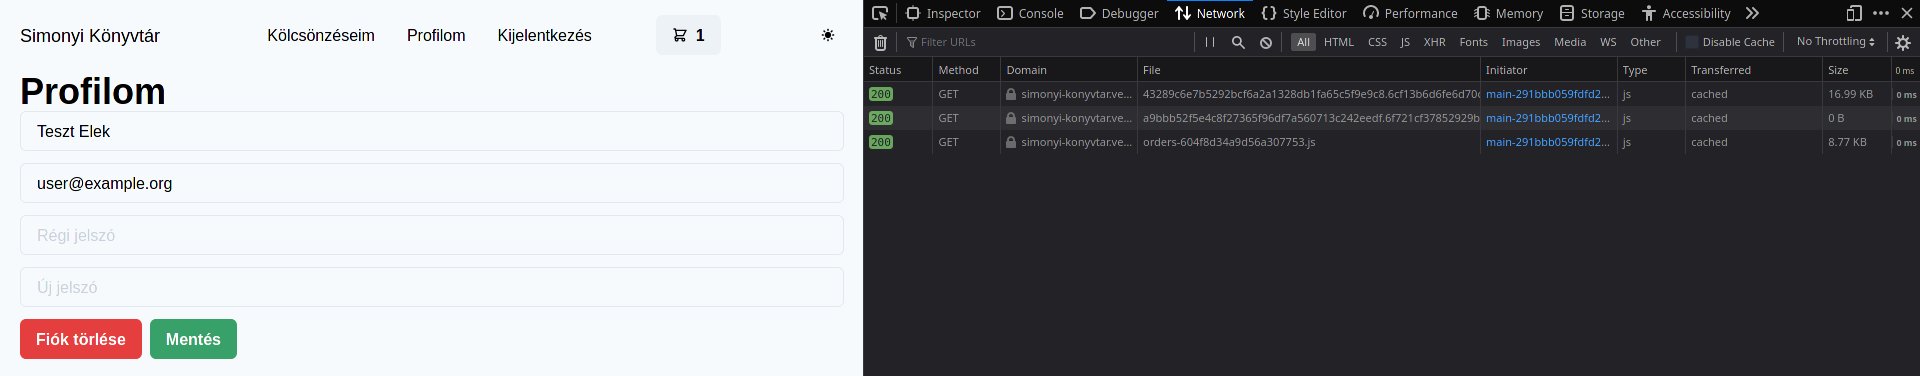
\includegraphics[width=150mm, keepaspectratio]{figures/next-link-cache.png}
  \caption{Next.js link prefetch}
  \label{fig:LinkPrefetch}
\end{figure}

\subsection{Optimistic UI update SWR-rel}

Egy másik, manapság gyakran alkalmazott módszer az úgynevezett Optimistic UI update.

Ennek lényege, hogy az oldalon megjelenített adat módosítása esetén előbb frissítjük a HTML tartalmat az új információval, minthogy a szervertől
pozitív választ kaptunk volna.

Nagy előnye a módszernek, hogy nem kell várni az esetlegesen sokáig tartó backend-oldali műveletekre, ami máskülönben ``befagyasztaná'' az alkalmazásunk
felületét. Fontos megjegyzés viszont, hogy navigációt nem érdemes így kezelni, mivel az esetleges hibákról nehéz értesíteni a felhasználót
és az esetleges inkonzisztens adatokkal nagyban csökkenthetjük a felhasználói élményt.

Az \lstinline|SWR| könyvtárat használva rendkívül egyszerűen valósíthatjuk meg ezt a funkcionalitást. A \lstinline|useSWR| hook által hozzáférésünk
van egy \lstinline|mutate| függvényhez, ami az általunk lekért erőforráshoz van kötve.

Ennek segítségével bármikor tudjuk módosítani a képernyőn megjelent adatainkat.
Ezt az SWR ezután validálja a POST kérésünk által visszaadott eredménnyel, és ha egyezik,
a belső állapotot is megváltoztatja, ha pedig eltérést tapasztal, akkor a korábbi állapotot őrzi meg és jeleníti meg a képernyőn.

\begin{lstlisting}[caption=Optimistic UI update megvalósítása]
export default function CategoriesIndexPage() {
  const hasAccess = useRequireRoles([userrole.ADMIN])
  if (!hasAccess) {
    return <ErrorPage statusCode={401} message="Nincs megfelelő jogosultságod!" />
  }
  const [newCategory, setNewCategory] = useState("")
  const { data, error, mutate } = useSWR<Category[]>("/api/categories", fetcher)

  const toast = useToast()

  if (error) return <Text fontSize="lg">Nem sikerült betölteni a kategóriákat</Text>
  if (!data) return <Loading />

  async function handleDelete(cat: Category) {
    // handle deleting a category
  }

  async function handleAddCategory(event: FormEvent) {
    event.preventDefault()
    const category: CategoryCreateInput = { name: newCategory }
    const res = await fetch("/api/categories", {
      method: "POST",
      body: JSON.stringify(category),
      headers: {
        "Content-Type": "application/json",
      },
    })
    if (res.ok) {
      setNewCategory("")

      mutate(async (categories) => {
        const newCategory = await res.json()

        return [newCategory, ...categories.slice(1)]
      })
    }
  }

  async function handleEditCategory({ id, name }) {
    // handle editing a category
  }

  return (
    <>
      <form onSubmit={handleAddCategory}>
        <Flex direction="row" mb={6}>
          <FormControl mr={4} flex="1">
            <Input
              isRequired
              placeholder="Új kategória"
              value={newCategory}
              onChange={(e: FormEvent<HTMLInputElement>) =>
                setNewCategory(e.currentTarget.value)
              }
            />
          </FormControl>
          <Button type="submit">Hozzáadás</Button>
        </Flex>
      </form>
      <Heading as="h1">Kategóriák</Heading>
      {data && (
        <CategoryList
          data={data}
          handleDelete={handleDelete}
          handleEdit={handleEditCategory}
        />
      )}
    </>
  )
}

\end{lstlisting}

\subsection{Page layout megvalósítása}

Az alkalmazásban a felső navigációs sávot és az alsó footer-t szerettem volna minden oldalon megjeleníteni.

Ehhez az egyik lehetőség, hogy minden aloldalba beillesztem ezt a két komponenst, azonban ez sok kódduplikációhoz és esetenként
inkonzisztens megjelnéshez vezetne.

Szerencsére a Next.js-ben lehetőségünk van egy központi layout kialakítására, ami azután minden oldalunk használni fog. Ehhez nem kell
mást tennünk, mint az \lstinline|src/pages| mappában létrehozni egy \lstinline|_app.tsx| nevű fájlt és itt implementálni az általunk
kívánt layout-ot.

\begin{lstlisting}[caption=Minden oldalra kiterjedő layout alkalmazása Next.js keretrendszerben]
import { Box, ChakraProvider } from "@chakra-ui/react"
import { AppProps } from "next/app"
import dynamic from "next/dynamic"
import Head from "next/head"

import { Container } from "components/Container"
import Footer from "components/Footer"

const Navbar = dynamic(() => import("components/Navbar"), { ssr: false })

const App = ({ Component }: AppProps) => {
  return (
    <>
      <Head>
        <title>Simonyi Könyvtár</title>
        <meta property="og:title" content="Simonyi Könvtár" key="title" />
        <meta lang="hu" />
      </Head>
      <ChakraProvider>
        <Container>
          <Navbar />
          <Box flex="1" width="100%" px={5} maxW="6xl">
            <Component />
          </Box>
          <Footer />
        </Container>
      </ChakraProvider>
    </>
  )
}

export default App
\end{lstlisting}

A fenti kódrészletben az \lstinline|App| komponens bemeneti paramétereiben lévő \lstinline|Component| reprezentálja az oldalanként
dinamikusan változó tartalmat. Az itt szereplő \lstinline|Container| komponens egy \lstinline|flexbox| konténer, aminek segítségével
a footer akkor is az oldal aljához tapad, ha a felette lévő tartalom nem tölti ki teljesen a képernyőt.


\section{Kódmegosztás}


\section{Képfeltöltés}

A könyvekhez lehetősév van borítóképet feltölteni, ezeket azonban valahol tárolni is kell.

Ennek a tárolására az Amazon S3 szolgáltatását választottam. A csatolt képet a frontend először elküldi a backendnek,
majd az az \lstinline|aws-sdk| könyvtárat használva feltölti a képet az S3 bucket-be, az adatbázisba csak a képet
azonosító generált kerül be. Így lehetőségünk van a képek egyszerű és adatbázisfüggetlen kezelésére.

\begin{figure}[!ht]
  \centering
  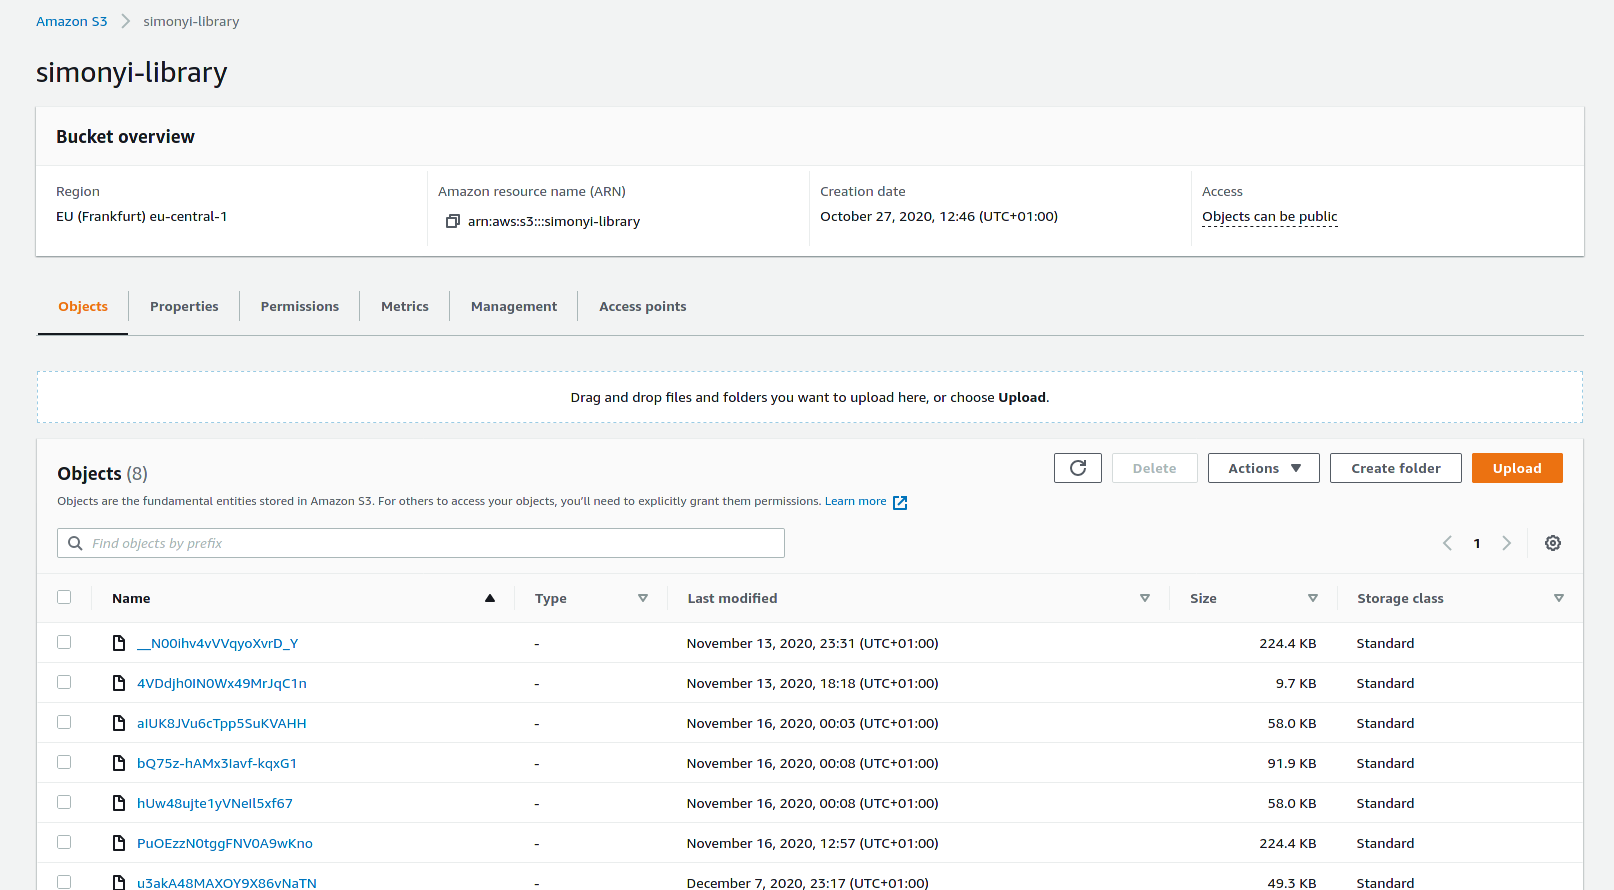
\includegraphics[width=125mm, keepaspectratio]{figures/s3-dashboard.png}
  \caption{Amazon S3 konzol}
  \label{fig:S3Console}
\end{figure}

\chapter{Az alkalmazás működése}

\section{Authentikáció}

A felhasználók magukat egy email-jelszó párossal tudják azonosítani, melyet regisztrációkor adhatnak meg.

A regisztráció kezelésénék két dologra kellett figyelmet fordítanom: egy email cím csak egyszer szerepelhessen
az adatbázisban, valamint a jelszót megfelelő módon tároljuk az adatbázisban.

Az első kritériumra megoldásként szolgál az adatbázisban az email mező egyedivé tétele, valamint a regisztráció során
a megadott emailcím ellenőrzése.

A jelszó biztonságos tárolása érdekében azt regisztráció során hash-elve mentem el az adatbázisba, erre az \lstinline|argon2| könyvtárat
használtam fel.

\subsection{Megvalósítás}

A session kezeléshez a \lstinline|passport| könyvtárat és cookie alapú megoldást használtam. Ennek során a felhasználót a böngészőben
tárolt cookie információ azonosítja, amit backenden ellenőrzi tudunk.

A frontenden történő ellenőrzéshez egy hook-ot készítettem, mellyel ellenőrzhető, hogy a felhasználó be van-e jelentkezve.

\begin{lstlisting}[caption=Authentikáció hook]
export function useUser() {
  const { data, mutate } = useSWR<{ user: User }>("/api/user", fetcher)
  const loading = !data
  const user = data?.user
  return [user, { mutate, loading }] as const
}
\end{lstlisting}

\section{Authorizáció}

Az alkalmazás megfelelő használata érdekében szükséges volt bizonyos funkciók elérésének szűkítésére. Ehhez a role-based access control
megoldást választottam, mely alapján a felhasználókat különböző kategórákba tudjuk besorolni, majd ezeknek a kategóriáknak adunk jogosultságokat.

Ennek megfelelően három jogosultság-kategóriát hoztam létre: \lstinline|BASIC|, \lstinline|ADMIN| és \lstinline|EDITOR|.

A \lstinline|BASIC| felhasználók képesek foglalást leadni és a sajátjaikhoz megjegyzést fűzni, valamint a hozzájuk tartozó foglalásokat listázni.

Az \lstinline|EDITOR| jogosultsággal rendelkezők ezen felül képesek az egyes foglalások állapotát állítani, valamint bármyely foglaláshoz
megjegyzést fűzni.

Az \lstinline|ADMIN| joggal rendelkezők a fentieken kívül képesek könyvek és kategóriák hozzáadására, törlésére és szerkesztésére.

\subsection{Megvalósítás}

A kódbázison belül a frontenden és backendes is szükséges elleőrizni a megfelelő jogosultságokat.

A backenden ehhez létrehoztam egy middleware-t, amely a már bejelentkezett emberek jogosultságát ellenőrzi.
\begin{lstlisting}[caption=Authorizáció middleware]
const requireRole = (...roles: userrole[]) => {
  return (req: NextApiRequest, res: NextApiResponse, next: NextHandler) => {
    if (roles.some(it => it === req.user.role)) {
      return next()
    } else {
      return res.status(401).json({ message: "Nincs megfelelő jogosultságod" })
    }
  }
}
\end{lstlisting}

A frontenden történő validáció esetén két forgatókönyv lehetséges: egy teljes oldal vagy az oldalon belül bizonyos komponensek
elrejtése a felhasználó elől.

Az előbbi kezelésére létrehoztam egy React hook-ot, amivel az oldalak megjelenítését tudjuk kontrollálni.

\begin{lstlisting}[caption=Authorizációs hook és használata]
// src/lib/hooks.tsx
export function useRequireRoles(roles: userrole[] = []) {
  const [user] = useUser()

  return roles.some((it) => it === user?.role)
}

// src/pages/admin/index.tsx
const hasAccess = useRequireRoles([userrole.ADMIN, userrole.EDITOR])
if (!hasAccess) {
  return <ErrorPage statusCode={401} message="Nincs megfelelő jogosultságod!" />
}
\end{lstlisting}

Az oldalon belüli bizonyos tartalmak elrejtésére készítettem egy komponenst, ami a tartalmát a felhasználó jogosultsági szintjének
megfelelően jeleníti csak meg.

\begin{lstlisting}[caption=Authorizáció komponens és használata]
// src/components/HasRole.tsx
export default function HasRole({ roles, children }: Props) {
  const [user] = useUser()
  const hasRole = roles.some((it) => it === user?.role)

  return <>{hasRole && children}</>
}

// src/components/Navbar.tsx
<HasRole roles={[userrole.ADMIN, userrole.EDITOR]}>
  <NextLink href="/admin">
    <Link>Admin</Link>
  </NextLink>
</HasRole>
\end{lstlisting}

A fenti módszerek alkalmazásásval egy robosztus jogosultság-kezelő megoldást sikerült implementálnom a szoftverbe.

\section{Könyvek listázása}

A kezdőoldalon az elérhető könyveket tudjuk listázni egy rácsszerkezetben.
Itt látható a könyvöz kapcsolt borítókép, a könyv címe, szerzője és kategóriái.

\begin{figure}[!ht]
  \centering
  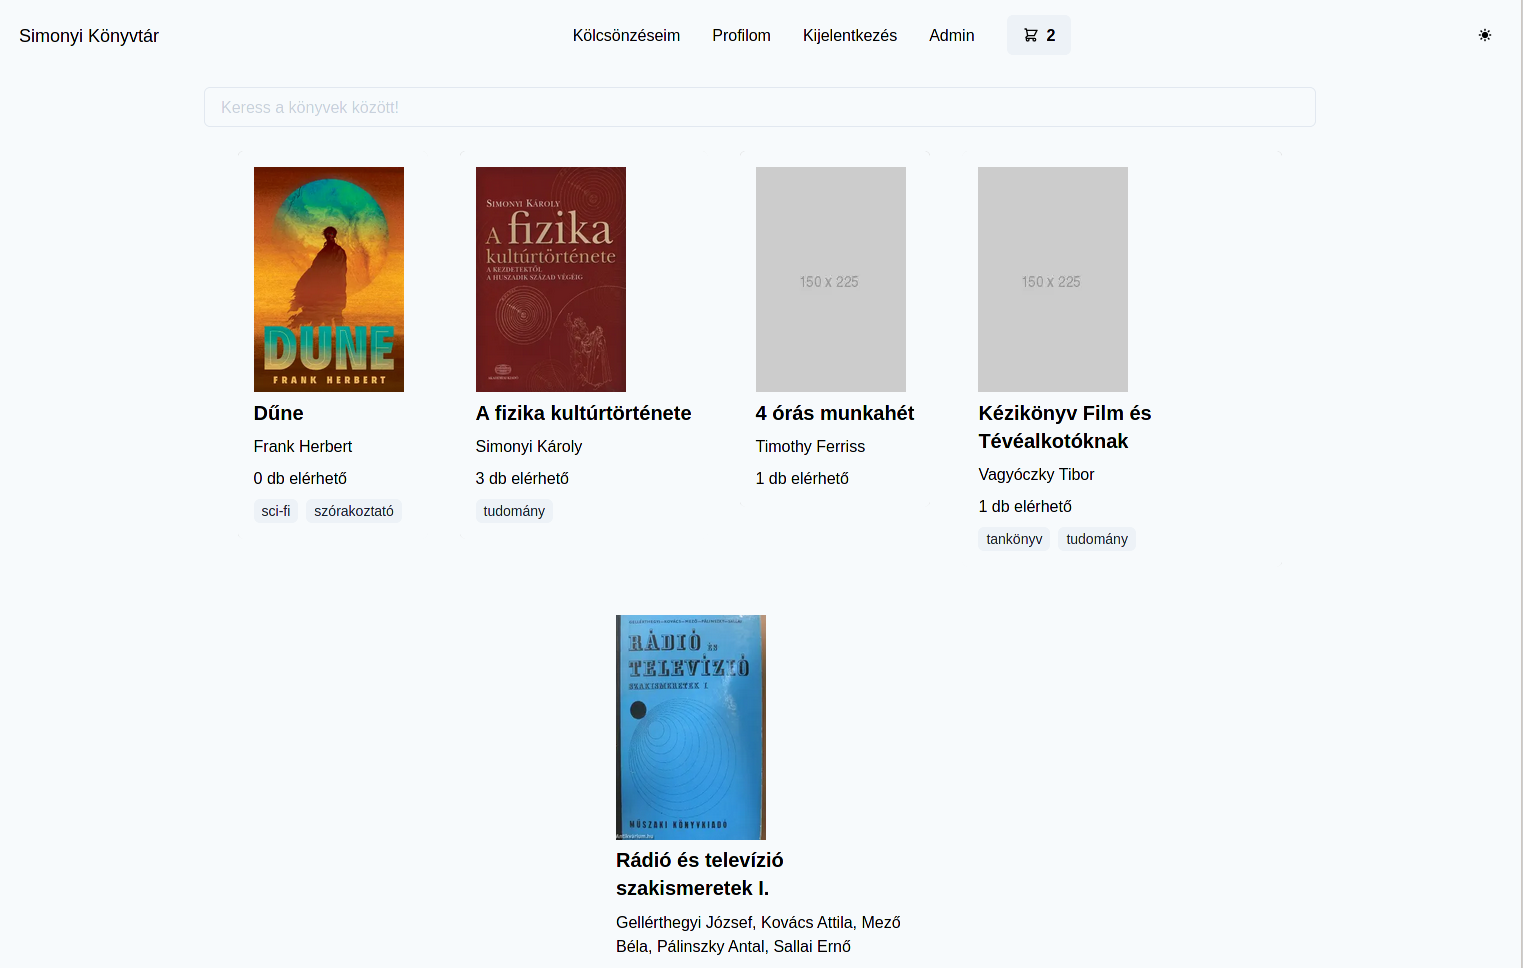
\includegraphics[width=150mm, keepaspectratio]{figures/index.png}
  \caption{Az alkalmazás kezdőlapja}
  \label{fig:IndexPage}
\end{figure}

\subsection{Részletes nézet}

A főoldalon egy könyvre kattintva megkapjuk annak részletes nézetét. Itt láthatjuk az összes hozzá tartozó információt, valamint
lehetőségünk van a könyv kosárba helyezésére (feltéve, hogy van belőle elérhető példány).

\begin{figure}[!ht]
  \centering
  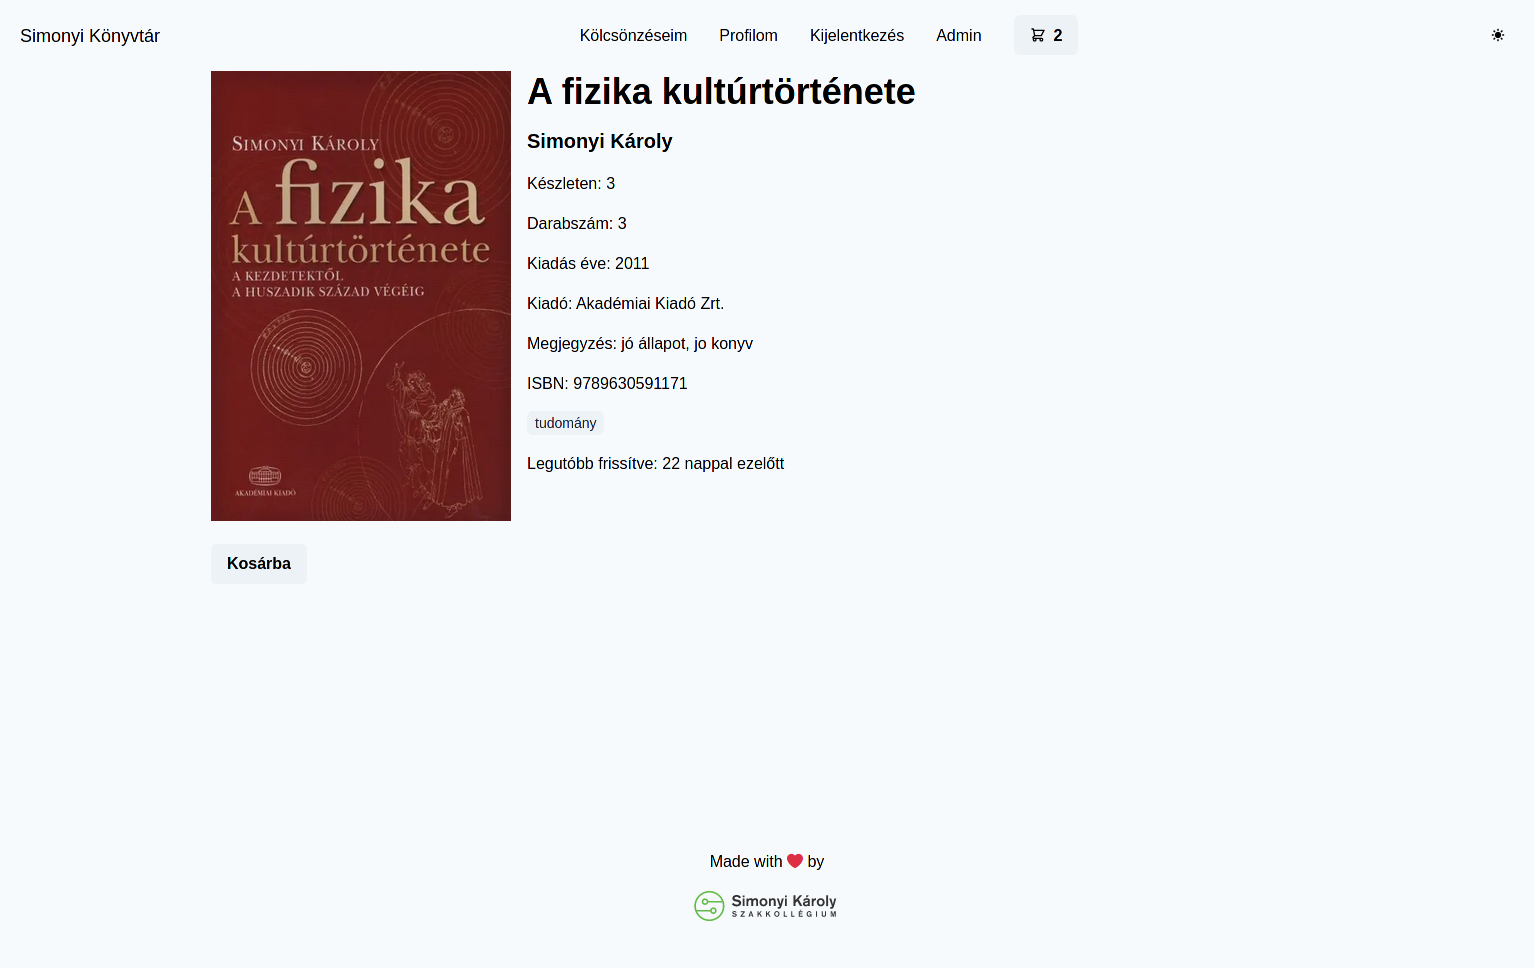
\includegraphics[width=100mm, keepaspectratio]{figures/book-detail-view.png}
  \caption{Könyv részletes nézete}
  \label{fig:BookDetailView}
\end{figure}

\subsection{Keresés a könyvek között}

A főoldalon tudunk a meglévő könyvek közötti kulcsszavas keresésre. Ezt a PostgreSQL Full Text Search funkciójával implementáltam.

Ehhez szükséges volt létrehozni az indexeléshez szükséges oszlopot a \lstinline|Book| táblán, ami alapján az adatbázismotor a kersést
el tudja végezni.

\begin{lstlisting}[caption=A kereséshez szükséges SQL utasítások]
ALTER TABLE "Book"
ADD COLUMN document tsvector;
update "Book"
set document = to_tsvector(title || ' ' || author || ' ' || publisher || '' || notes);

ALTER TABLE "Book"
ADD COLUMN document_with_idx tsvector;
update "Book"
set document_with_idx = to_tsvector(title || ' ' || coalesce(author, '') || ' ' || coalesce(publisher, '') || '' || coalesce(notes, ''));
CREATE INDEX document_idx
ON "Book"
USING GIN(document_with_idx);

ALTER TABLE "Book"
  ADD COLUMN document_with_weights tsvector;
update "Book"
set document_with_weights = setweight(to_tsvector(title), 'A') ||
  setweight(to_tsvector(coalesce(author, '')), 'B') ||
  setweight(to_tsvector(coalesce(publisher, '')), 'C') ||
  setweight(to_tsvector(coalesce(notes, '')), 'D');
CREATE INDEX document_weights_idx
  ON "Book"
  USING GIN (document_with_weights);

CREATE FUNCTION book_tsvector_trigger() RETURNS trigger AS $$
begin
  new.document :=
  setweight(to_tsvector('english', coalesce(new.title, '')), 'A')
  || setweight(to_tsvector('english', coalesce(new.author, '')), 'B')
  || setweight(to_tsvector('english', coalesce(new.publisher, '')), 'C')
  || setweight(to_tsvector('english', coalesce(new.notes, '')), 'D');
  return new;
end
$$ LANGUAGE plpgsql;

CREATE TRIGGER tsvectorupdate BEFORE INSERT OR UPDATE
    ON "Book" FOR EACH ROW EXECUTE PROCEDURE book_tsvector_trigger();

\end{lstlisting}

A keresés implementálásához szükséges volt még egy egyedi lekérdezés írása, ugyanis a Prisma jelenleg nem támogatja a \lstinline|tsvector|
alapú keresést. Ehhez az alábbi megoldást használtam a backenden.

\begin{lstlisting}[caption=Könyvek közti keresés megvalósítása]
const sql = escape(`
select id, title, author, "stockCount", "updatedAt", image
from "Book"
where document_with_idx @@ plainto_tsquery('%s')
order by ts_rank(document_with_idx, plainto_tsquery('%s')) desc;`, term)
const books = await db.$queryRaw(sql)
\end{lstlisting}

Alapesetben ha elkezdünk a keresőmezőbe gépelni, a frontend minden egyes leütés után kérést intéz a backend felé.
Ez azonban felesleges forgalmat és adatbáziselérést okoz, ezért az input késleltetésére a \lstinline|use-debounce| pagckage-et használtam.

\begin{lstlisting}[caption=A keresést megvalósító kódrészlet a frontenden]
const [term, setTerm] = useState("")
const { data, error } = useSWR<BookWithCategories[]>(`/api/books?q=${term}`, fetcher)
const debounced = useDebouncedCallback((value) => setTerm(value), 500)

return (
  <Input
    placeholder="Keress a könyvek között!"
    mt="1rem"
    onChange={(e) => debounced.callback(e.target.value)}
  />
  {/* ... */}
)
\end{lstlisting}

\section{Foglalási folyamat}

Az alkalmazás legfontosabb eleme a könyvek foglalásának nyomonkövetése. Az alábbi ábrán ennek a folyamatát foglaltam össze.

\begin{figure}[!ht]
  \centering
  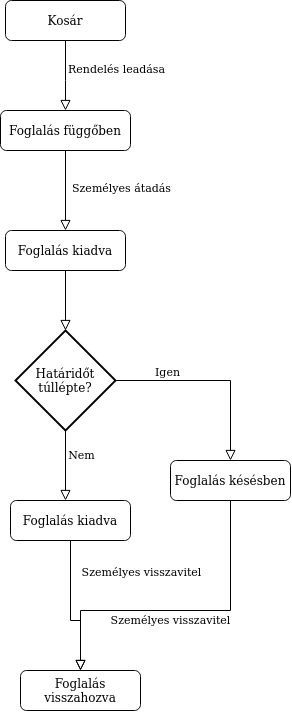
\includegraphics[width=50mm, keepaspectratio]{figures/order-flowchart.png}
  \caption{Rendelés leadásának menete}
  \label{fig:OrderChart}
\end{figure}

Egy foglalás leadása esetén a könyvből elérhető darabszámot is frissíteni kell. Ez több tábla szimultán módosításával jár,
viszont az inkonzisztencia elkerülése érdekében ennek teljesítenie kell az ACID elveket.

Mivel a Prisma jelenleg nem támogatja ilyen komplex módosítások egy utasításban történő végrehajtását, annak Transaction API
funkcióját használtam. Ennek segítségével több, egymástól független adatbázismódosítást lehet egyetlen tranzakcióba csomagolni,
így vagy minden kívánt módosítás érvényesül, vagy egyik sem.

\begin{lstlisting}[caption=Transaction API használata kölcsönzés létrehozásakor]
const createOrder = db.order.create({
  data: {
    returnDate,
    user: {
      connect: { id: userId },
    },
    books: {
      create: books.map(it => ({
        quantity: it.quantity,
        books: {
          connect: { id: it.id },
        }
      })),
    }
  },
})

const bookUpdates = books.map(book => {
  const bookUpdate = db.book.update({
    where: { id: book.id },
    data: {
      stockCount: { decrement: book.quantity }
    }
  })
  return bookUpdate
})

const [order] = await db.$transaction([createOrder, ...bookUpdates])
\end{lstlisting}

A fenti kódrészlet három fő utasításra bontható: létrehozza az \lstinline|Order| táblában az új bejegyzést a foglalásra,
beszúrja az \lstinline|Order| és \lstinline|Book| táblák közti kapcsolatot megteremtő kapcsolótáblába a megfelelő rekordokat,
valamint frissíti a \lstinline|Book| táblában lévő könyvek elérhető darabszámát.

\subsection{Kosár}

A könyv részletes nézetében lehetőség van a kosárba helyezésre. Ennek a tartalmát a felső navigációs sávon lévő bevásárlókosár
ikonra kattintva lehet megtekinteni.

\begin{figure}[!ht]
  \centering
  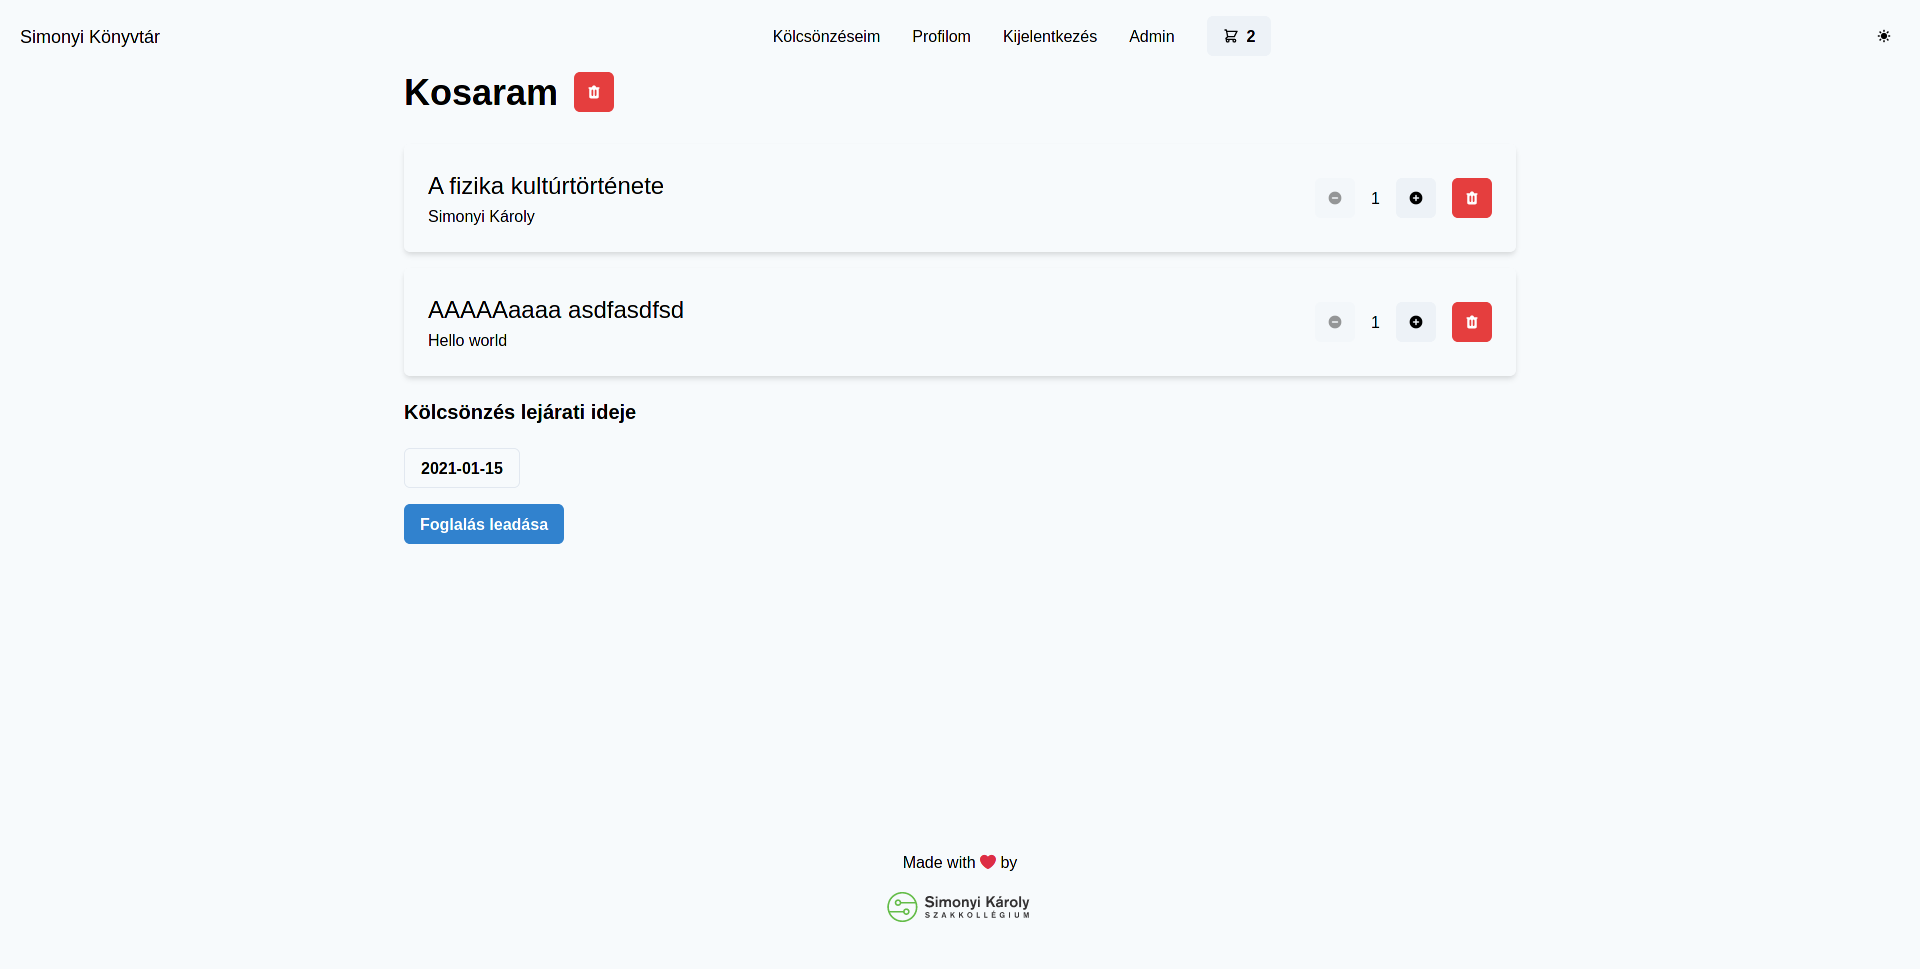
\includegraphics[width=150mm, keepaspectratio]{figures/cart.png}
  \caption{Kosár oldal}
  \label{fig:CartPage}
\end{figure}

Itt lehetőség van az egyes könyvek darabszámának állítására, illetve a kosár tartalmának módosítására.

Ezután a felhasználó ki tudja választani, hogy meddig szeretné kiválasztani a könyveket, majd a ``Foglalás leadása'' gombra kattintva
véglegesítheti azt.

A kosár adatainak tárolására a böngésző Local Storage funkcióját használtam.

Ezen megoldás előnye, hogy bejelentkezés nélkül is hozzáadhatóak könyvek és egyszerűbbé teszi az adatbázisstruktúrát.
Hátránya azonban, hogy nem kezeli a különböző böngészők (pl. asztali és mobil kliens) közötti szinkronizációt. Mivel ez utóbbi a
követelmények kidolgozása közben nem merült fel, így az egyszerűbb megoldás alkalmazása mellett döntöttem.

A kosár React-ban történő eléréséhez a \lstinline|use-persisted-state| könyvtárat vettem igénybe.

Segítségével több böngészőablakon keresztül is szinkronban tartható a kosárba helyezett könyvek,
valamint könyv hozzáadásakor illetve törlésekor automatikusan frissül minden megjelenített, kosárhoz kapcsolódó tartalom.

\subsection{Foglalás kezelése}

A foglalás leadás után a ``Kölcsönzéseim'' linkre kattintva tudjuk listázni azokat. Itt egy adott kölcsönzésre kattintva
léphetünk a részletes nézetre, ahol megjegyzéseket tudunk fűzni hozzá. Ez a funkció szolgál az átvételi időpont egyeztetésére,
problémák és egyéb igények megbeszélésére.

\begin{figure}[!ht]
  \centering
  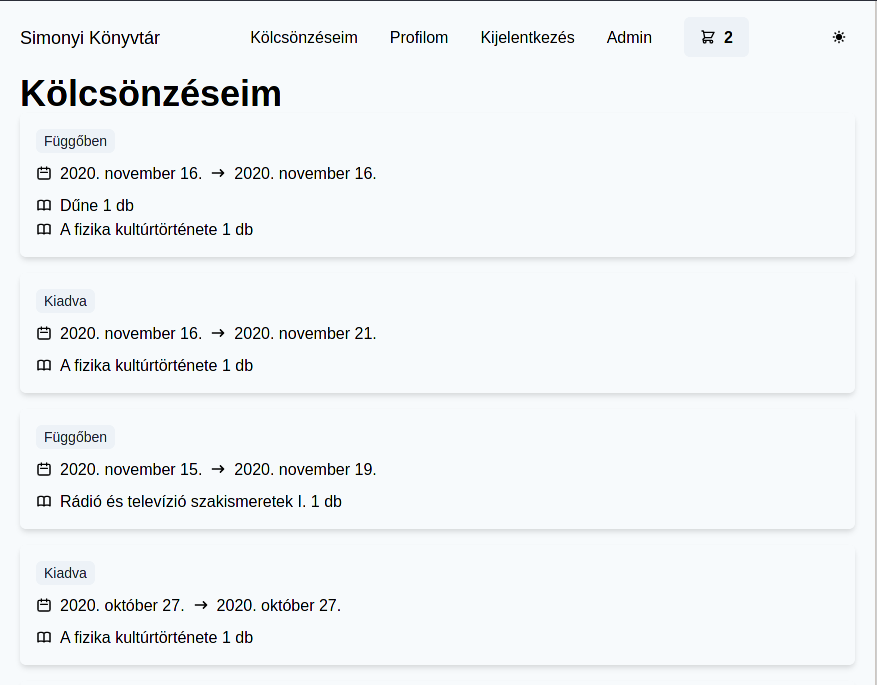
\includegraphics[width=150mm, keepaspectratio]{figures/orders-list.png}
  \caption{Kölcsönzések listázása}
  \label{fig:OrderList}
\end{figure}


\begin{figure}[!ht]
  \centering
  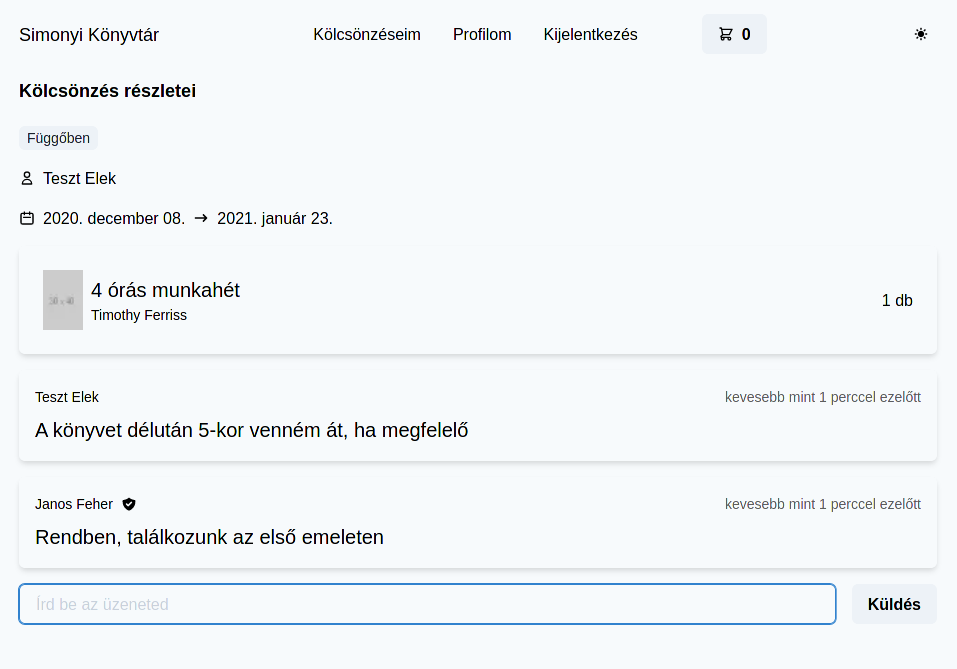
\includegraphics[width=150mm, keepaspectratio]{figures/order-detail.png}
  \caption{Kölcsönzés részletei kommentekkel}
  \label{fig:OrderDetail}
\end{figure}


\section{Admin funkciók}

Az \lstinline|ADMIN| illetve \lstinline|EDITOR| jogosultsággal rendelkező felhasználóknak lehetőségük van a rendszerben
lévő adatokat a webes felületről szerkeszteni. Ehhez a \lstinline|pages/admin| mappában külön oldalakat hoztam létre,
a backenden pedig a védett middleware-ekben valósítottam meg a funkciókat.

\subsection{Könyvek kezelése}

A könyveket egy listanézet foglalja össze. Itt lehetőség van az egyes elemek törlésére és szerkesztésére, valamint új
könyv hozzáadására. A szerkesztéshez és létrehozáshoz ugyanazt a komponenst használtam a kódduplikáció elkerülése érdekében.

\begin{figure}[!ht]
  \centering
  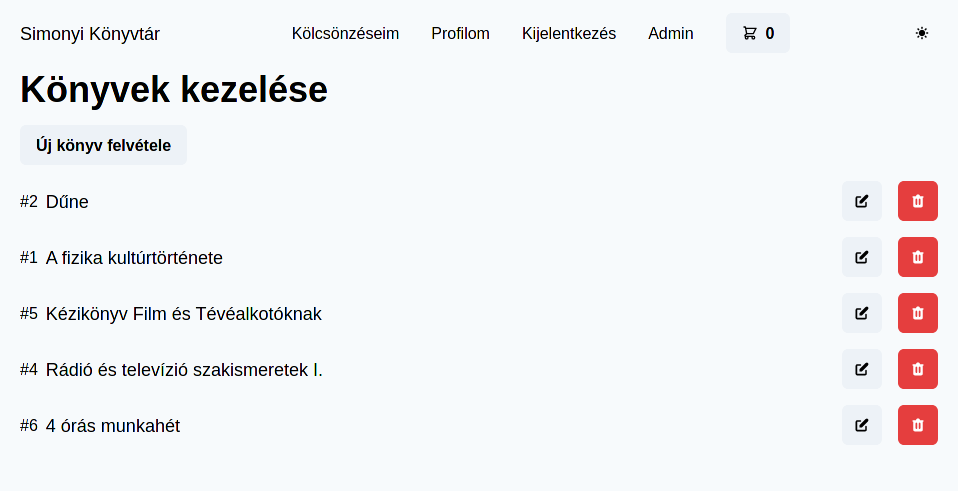
\includegraphics[width=100mm, keepaspectratio]{figures/book-admin-list.png}
  \caption{Könyvek listája az admin panelen}
  \label{fig:BookAdminList}
\end{figure}

\begin{figure}[!ht]
  \centering
  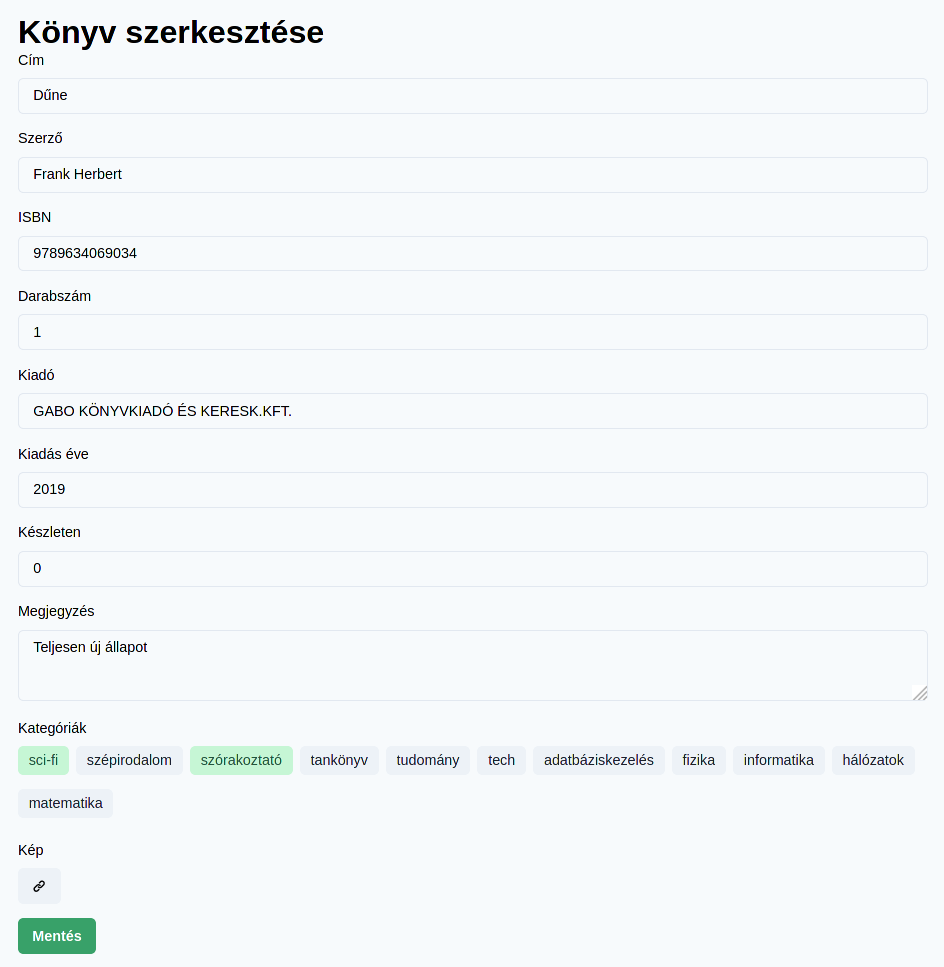
\includegraphics[width=100mm, keepaspectratio]{figures/book-edit.png}
  \caption{Könyv adatainak szerkesztése}
  \label{fig:BookEdit}
\end{figure}


\subsubsection{Fájlfeltöltés}

A könyvekhez opcionálisan megadható egy borítókép, amit a felhasználó a saját gépéről választhat ki.

Ennek a tárolására az Amazon S3 szolgáltatását választottam. A csatolt képet a frontend először elküldi a backendnek,
majd az az \lstinline|aws-sdk| könyvtárat használva feltölti a képet az S3 bucket-be, az adatbázisba csak a képet
azonosító generált kerül be. Így lehetőségünk van a képek egyszerű és adatbázisfüggetlen kezelésére.

\begin{figure}[!ht]
  \centering
  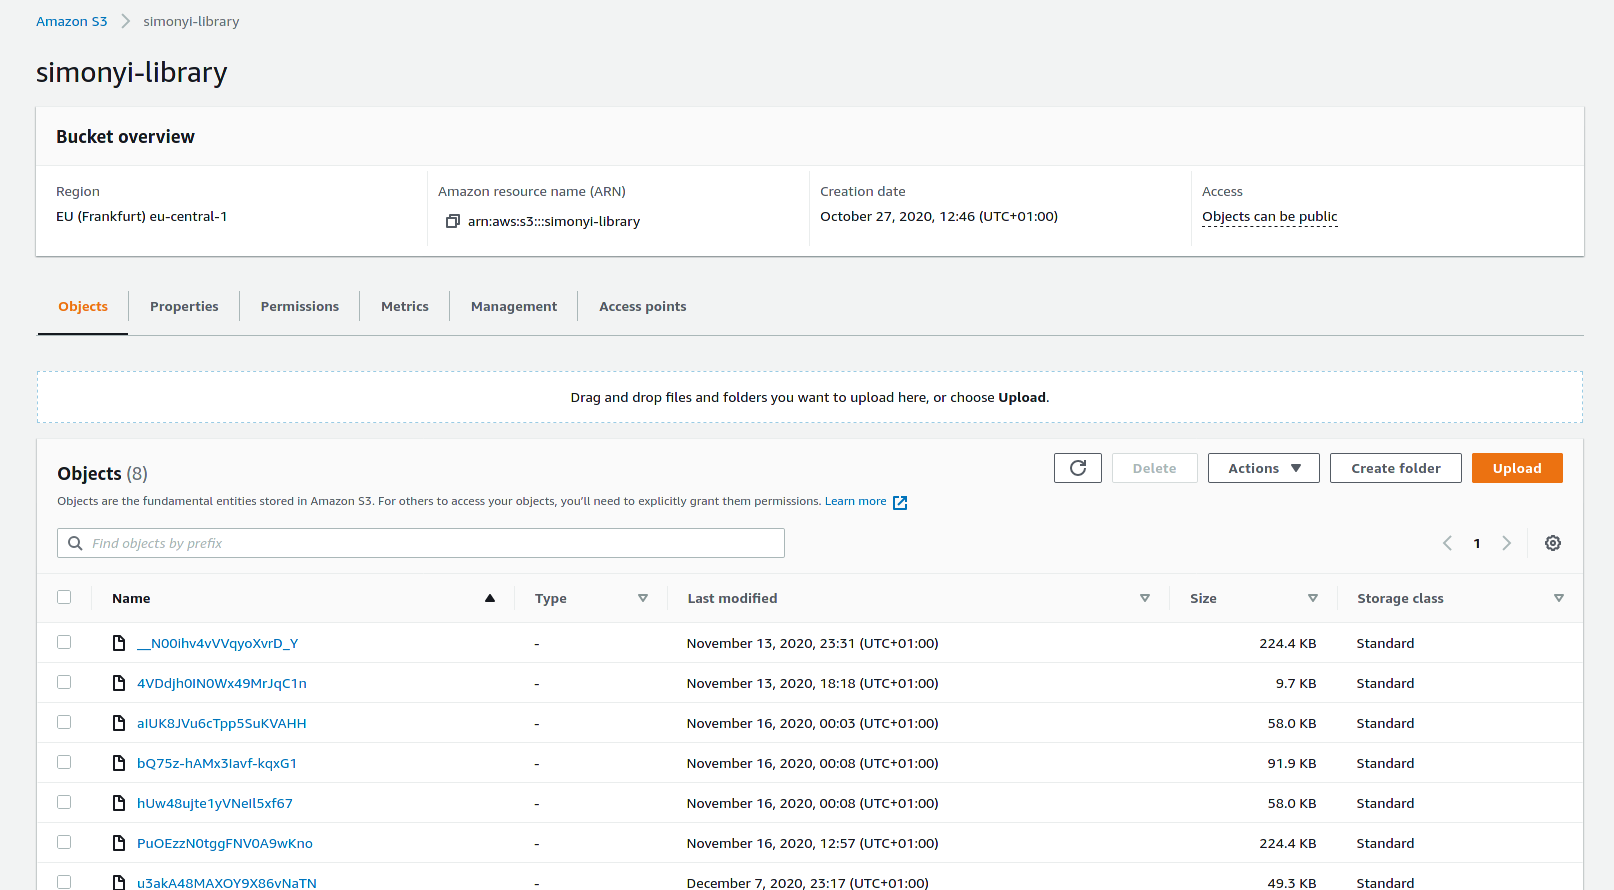
\includegraphics[width=125mm, keepaspectratio]{figures/s3-dashboard.png}
  \caption{Amazon S3 konzol}
  \label{fig:S3Console}
\end{figure}

\subsection{Kategóriák kezelése}

A kategóriákat egy összefoglaló oldalon lehet szerkeszteni és törölni. Egy elem eltávolítása esetén
minden hozzá kapcsolódó könyből is törlődik az adott kategória. Szerkesztés esetén egy felugró párbeszédablakban lehet
megadni az új nevet.

\begin{figure}[!ht]
  \centering
  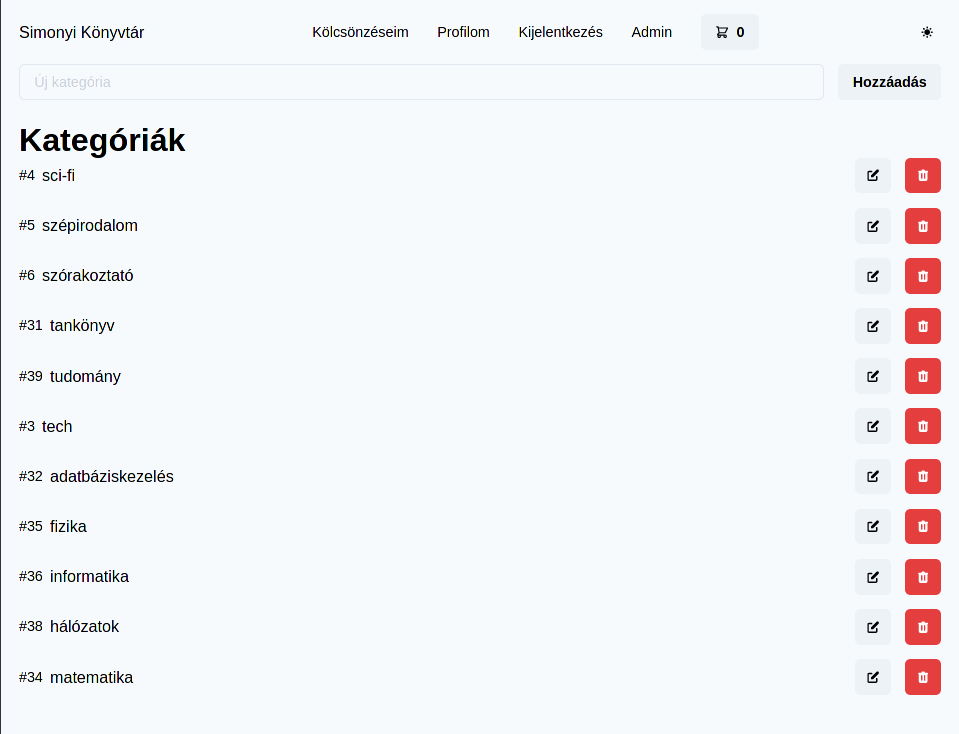
\includegraphics[width=150mm, keepaspectratio]{figures/category-admin-list.png}
  \caption{Kategóriák kezelése oldal}
  \label{fig:CategoryAdmin}
\end{figure}

\subsection{Foglalások kezelése}

% TODO
A foglalásokat egy központi oldalon lehet listázni a fontosabb információkkal.

\begin{figure}[!ht]
  \centering
  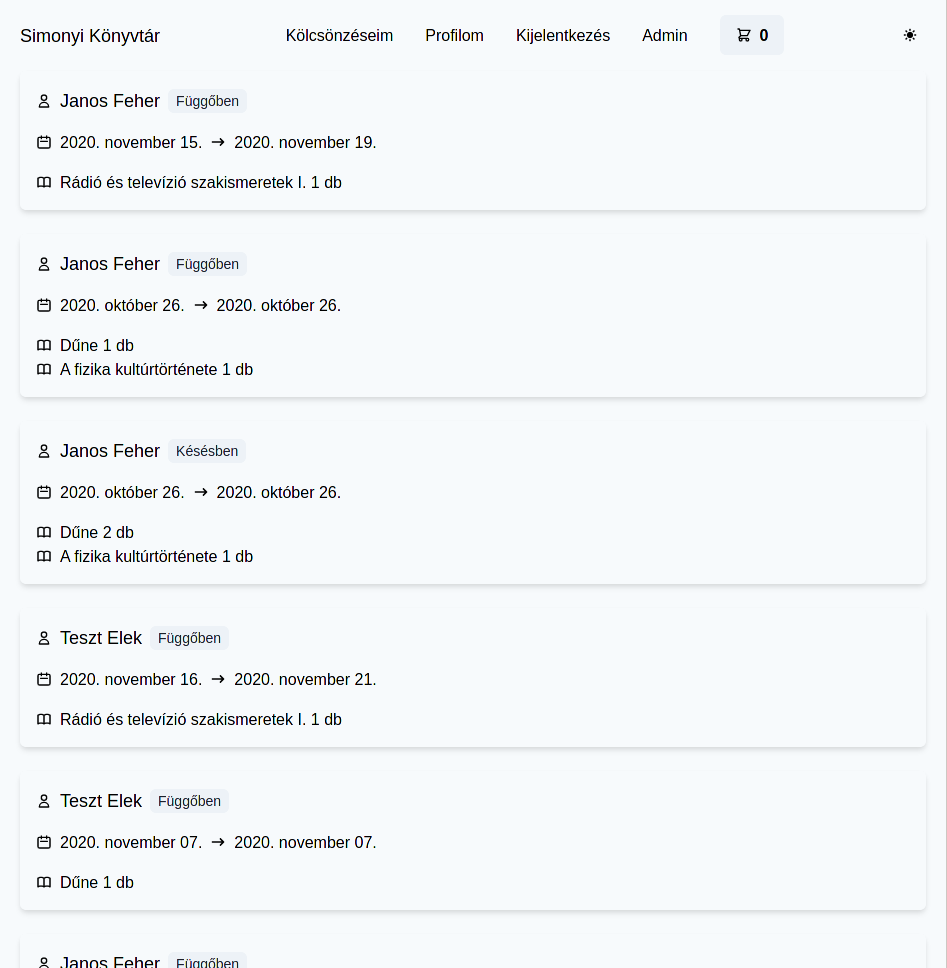
\includegraphics[width=150mm, keepaspectratio]{figures/order-admin-list.png}
  \caption{Összes foglalás listázása az adminok számára}
  \label{fig:OrderAdminList}
\end{figure}

Egy kölcsönzésre kattintva a részletes nézet jelenik meg. Itt az arra jogosultaknak lehetősége van az állapot módosítására vagy
a foglalás törlésére. Szintén itt van lehetőség minden arra jogosultnak a foglaláshoz hozzászólást fűzni.

\begin{figure}[!ht]
  \centering
  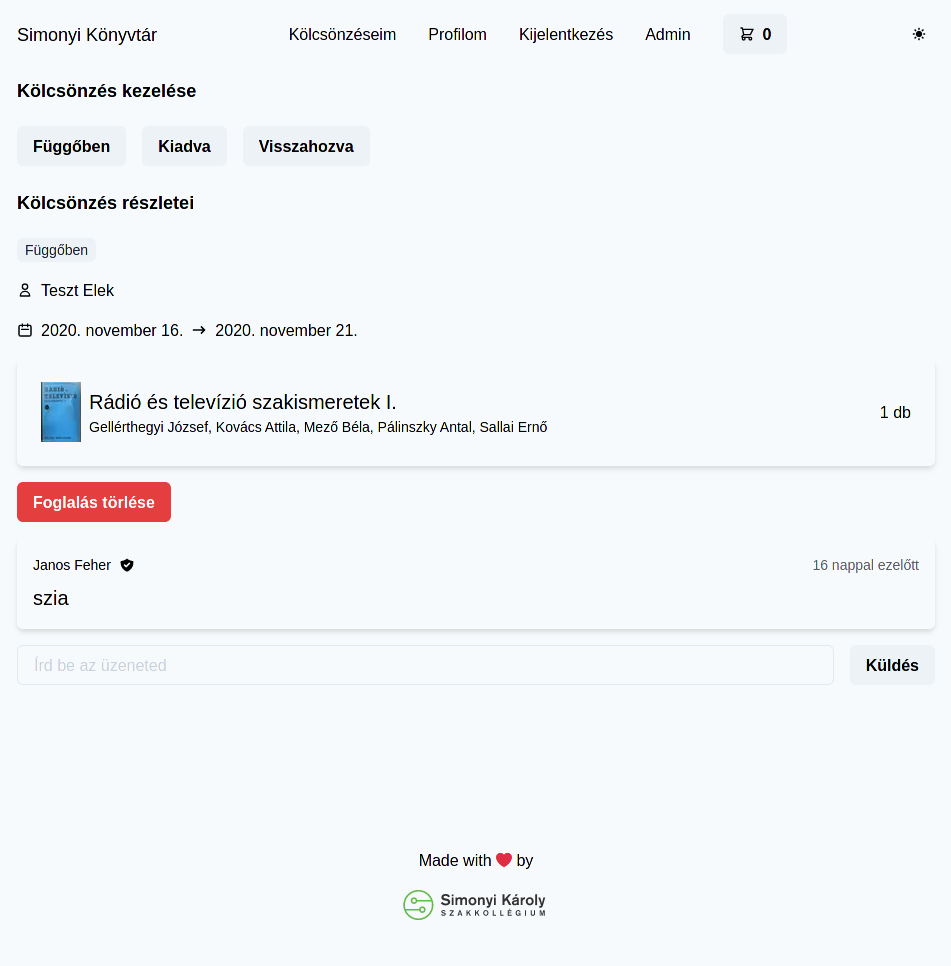
\includegraphics[width=150mm, keepaspectratio]{figures/order-admin-detail.png}
  \caption{Foglalás részletes nézete az adminok számára}
  \label{fig:OrderAdminDetail}
\end{figure}

Ha az állapot ``Visszahozva'' státuszra módosul, a foglalás leadásához hasonlóan firssülnek a könyvhöz tartozó elérhetőségi adatok.

\section{Adaptív UI}

A felület fejelsztése közben fontos volt, hogy minden oldal megfelelően működjön mobil képernyőkön is.
A Chakra UI szerencsére első kézből támogatja ezt a Responsive Styles funkciójának köszönhetően.

Ennek segítségével egy Chakra komponens tulajdonságait egy tömbben tudjuk megadni, ahol minden elem egy adott képernyőmérethez
fog társulni.

\begin{lstlisting}[caption=Chakra UI Responsive Styles használata]
<Flex direction={["column", null, "row"]}>
  <Box mr={4}>
    <NextImage
      src={
        book.image
          ? `${process.env.NEXT_PUBLIC_S3_URL}/${book.image}`
          : "https://via.placeholer.com/200x300"
      }
      width={300}
      height={450}
    />
  </Box>
  {/* Other content */}
</Flex>
\end{lstlisting}

\begin{figure}[!ht]
  \centering
  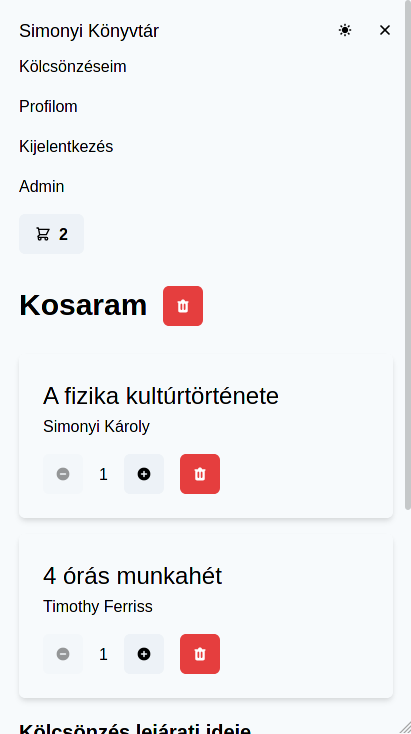
\includegraphics[width=75mm, keepaspectratio]{figures/cart-mobile.png}
  \caption{Kosár oldal mobil képernyőn, nyitott menüvel}
  \label{fig:CartMobile}
\end{figure}

\section{Dark Mode}

A Chakra UI egyik rendkívül hasznos tulajdonsága, hogy elsőrendű dark mode támogatással rendelkezik, és valamennyi komponensnek
létezik sötét módú variánsa.
Ennek segítségével gombnyomásra válthatunk a világos és sötét módok között.

\begin{figure}[!ht]
  \centering
  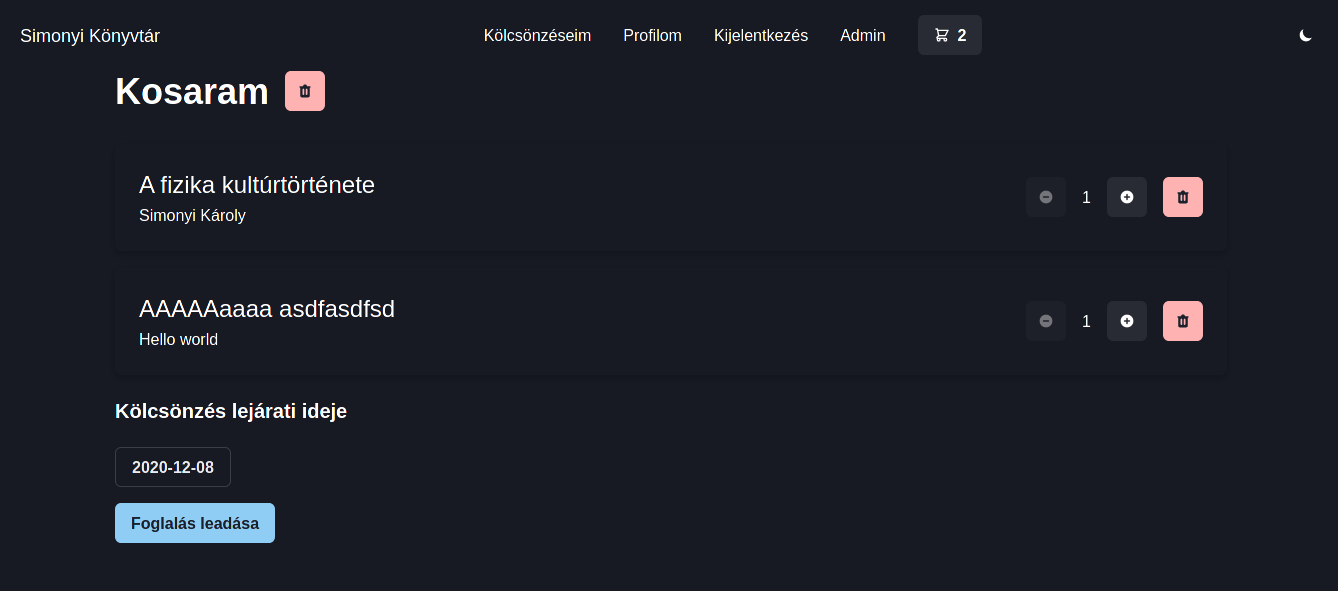
\includegraphics[width=150mm, keepaspectratio]{figures/dark-mode.png}
  \caption{Sötét téma}
  \label{fig:DarkMode}
\end{figure}

\section{Validáció}

A felhasználó által szolgáltatott adatok minden esetben potenciális veszélyforrást jelenthetnek, legyen szó XSS támadásról
vagy az adatbázis struktúrájának integritásáról. Emiatt különösen fontos a backenden történő adatok megfelelő validációja.

Ezen adatok ellenőrzésére a \lstinline|yup| könyvtárat használtam. Segítségével definiálhatunk egy sémát, ami ellen
a felhasználó által megadott adatot validálhatjuk. Ezáltal a potenciális inkonzisztenciákat még az adatbázisba írás előtt
kiszűrhetjük és tudathatjuk a felhasználóval.

\begin{lstlisting}[caption=yup validációs séma a könyvekre]
export const BookSchema = yup.object().shape({
  title: yup.string().required(),
  author: yup.string(),
  count: yup.number(),
  stockCount: yup.number(),
  isbn: yup.string(),
  publisher: yup.string(),
  publishedAt: yup.number(),
  notes: yup.string(),
  image: yup.string(),
})
\end{lstlisting}

\chapter{CI/CD}

A Continuous Integration / Continuous Delivery egy manapság már általánosan használt módszer az alkalmazások folyamatos tesztelésére és publikálására.

A Simonyi Könyvtár esetében igyekeztem ezeket a megközelítéseket alkalmazni a fejlesztés és deploy esetében is.

\section{Continuous Integration}

A forráskód tárolására a GitHub-ot használtam, így CI megoldásnak evidens volt a GitHub Actions használata.

Ez esetben elegendő egy \lstinline|.yaml| fájlt elhelyezni a \lstinline|.github/workflows/| mappába elhelyezni, és egy \lstinline|git push|
parancs kiadása után automatikusan lefut a szkriptünk. Ennek az állapotát a GitHub repository webes felületén tudjuk követni.

\subsection{Statikus kódanalízis}

A fejlesztés során nagy segítséget nyújtanak azok az eszközök, amelyek segítségével a forráskódunkat még fordítás vagy futtatás
előtt ellenőrizni tudjuk.

A JavaScript világában ennek egyik szinte sztenderddé vált eszköze az \lstinline|eslint|, amely egy TypeScript-hez is használható linter.
Ennek segítségével ki tudjuk szűrni a nem használt kódrészleteket, valamint egységes formázást írhatunk elő a forráskódra, nagyban segítve
ezzel a közös munkát.

Az alkalmazásomban én is ezt a megoldást használtam, mely lokálist a \lstinline|yarn lint| parancs kiadásával lokálisan, valamint
a GitHub Actions build folyamataként automatikusan is futtatható.

\section{Continuous Delivery}

Az alkalmazás hostolására két szolgáltatást használtam.

A frontend és backend közös deploymentjéhez a Vercel-t választottam. Ez rendkívül egyszerűen integrálható a Next.js keretrendszerrel,
elegendő a GitHub repository-val összekötni és bármiféle extra konfiguráció nélkül elérhető lesz az alkalmazásunk egy \lstinline|git push| parancs kiadása után.

A Vercel felületén lehetőségünk van a deployment státuszát ellenőrizni, korábbi deploymentre visszaállni, illetve a Next.js 10-es verziójától kezdve
már különböző analitikák monitorozására is.

Az adatbázishoz a Heroku ingyenes PostgreSQL szolgáltatását vettem igénybe. Ebben az esetben elegendő az adatbázishoz kapott
connection string-et a Vercel felületén a környezeti változók között megadni, és az alkalmazásunk hozzáfér az adatbázisunkhoz.


% Acknowledgements
%~~~~~~~~~~~~~~~~~~~~~~~~~~~~~~~~~~~~~~~~~~~~~~~~~~~~~~~~~~~~~~~~~~~~~~~~~~~~~~~~~~~~~~
%----------------------------------------------------------------------------
\chapter*{\koszonetnyilvanitas}\addcontentsline{toc}{chapter}{\koszonetnyilvanitas}
%----------------------------------------------------------------------------

Szeretném megköszönni a segítséget és együttműködést a Simonyi Károly Szakkollégium elnökségének, akik támogattak a
projekt elkészítésében és megvalósításában.



% List of Figures, Tables
%~~~~~~~~~~~~~~~~~~~~~~~~~~~~~~~~~~~~~~~~~~~~~~~~~~~~~~~~~~~~~~~~~~~~~~~~~~~~~~~~~~~~~~
%\listoffigures\addcontentsline{toc}{chapter}{\listfigurename}
%\listoftables\addcontentsline{toc}{chapter}{\listtablename}


% Bibliography
%~~~~~~~~~~~~~~~~~~~~~~~~~~~~~~~~~~~~~~~~~~~~~~~~~~~~~~~~~~~~~~~~~~~~~~~~~~~~~~~~~~~~~~
\addcontentsline{toc}{chapter}{\bibname}
\bibliography{bib/mybib}


% Appendix
%~~~~~~~~~~~~~~~~~~~~~~~~~~~~~~~~~~~~~~~~~~~~~~~~~~~~~~~~~~~~~~~~~~~~~~~~~~~~~~~~~~~~~~
%----------------------------------------------------------------------------
\appendix
%----------------------------------------------------------------------------
\chapter*{\fuggelek}\addcontentsline{toc}{chapter}{\fuggelek}
\setcounter{chapter}{\appendixnumber}
%\setcounter{equation}{0} % a fofejezet-szamlalo az angol ABC 6. betuje (F) lesz
\numberwithin{equation}{section}
\numberwithin{figure}{section}
\numberwithin{lstlisting}{section}
%\numberwithin{tabular}{section}

A program forráskódja a \href{https://OmTheTurtle/simonyi-konyvtar}{GitHub}-on. A legfrisseb build pedig megtekinthető a \href{https://simonyi-konyvtar.vercel.app}{https://simonyi-konyvtar.vercel.app} oldalon.


%\label{page:last}
\end{document}
